%
% This is one of the samples from the lawtex package:
% http://lawtex.sourceforge.net/
% LawTeX is licensed under the GNU General Public License 
%
\providecommand{\documentclassflag}{}
\documentclass[12pt,\documentclassflag]{michiganCourtOfAppealsBrief}
%\documentclass{article}

% for striking a row in a table, see https://tex.stackexchange.com/a/265728/135718
\usepackage{tikz}
\usetikzlibrary{tikzmark}

\makeandletter% use \makeandtab to turn off

% allow footnote refs, see https://tex.stackexchange.com/a/35044/135718
\makeatletter
\newcommand\footnoteref[1]{\protected@xdef\@thefnmark{\ref{#1}}\@footnotemark}
\makeatother

% Use this to show a line grid-
% \usepackage[fontsize=12pt,baseline=24pt,lines=27]{grid}
% \usepackage{atbegshi,picture,xcolor} % https://tex.stackexchange.com/a/191004/135718
% \AtBeginShipout{%
%   \AtBeginShipoutUpperLeft{%
%     {\color{red}%
%     \put(\dimexpr -1in-\oddsidemargin,%
%          -\dimexpr 1in+\topmargin+\headheight+\headsep+\topskip)%
%       {%
%        \vtop to\dimexpr\vsize+\baselineskip{%
%          \hrule%
%          \leaders\vbox to\baselineskip{\hrule width\hsize\vfill}\vfill%
%        }%
%       }%
%   }}%
% }
%   \linespread{1}

\usepackage[modulo]{lineno}% use \linenumbers to show line numbers, see https://texblog.org/2012/02/08/adding-line-numbers-to-documents/

% from https://tex.stackexchange.com/a/313337/135718
\usepackage{enumitem,amssymb}
\usepackage{pdfpages}
\usepackage{extramarks}
\usepackage{fancyhdr}
\usepackage{extramarks}
\usepackage{hyperref}
\RequirePackage{xr}
\externaldocument{appendix}

\newlist{todolist}{itemize}{2}
\setlist[todolist]{label=$\square$}
\usepackage{pifont}
\newcommand{\cmark}{\ding{51}}%
\newcommand{\xmark}{\ding{55}}%
\newcommand{\done}{\rlap{$\square$}{\raisebox{2pt}{\large\hspace{1pt}\cmark}}%
\hspace{-2.5pt}}
\newcommand{\wontfix}{\rlap{$\square$}{\large\hspace{1pt}\xmark}}


% allow underscores in words
\chardef\_=`_% https://tex.stackexchange.com/a/301984/135718 

%%Citations
 
%The command \makeandletter turns the ampersand into a printable character, rather than a special alignment tab \makeandletter

\begin{document}
\singlespacing%

\citecase[Antisdale]{Antisdale v City of Galesburg, 420 Mich 265, 362 NW2d 632 (1984)}
\citecase[Bennett]{Bennett v Bennett, 197 Mich. App. 497; 496 N.W.2d 353 (1992)}
\citecase[Berger]{Berger v Berger, 747 N.W.2d 336; 277 Mich. App. 700 (2008)}
\citecase[Briggs]{Briggs Tax Service, LLC v Detroit Pub. Schools, 485 Mich 69; 780 NW2d 753 (2010)}
\citecase[CAF v STC]{CAF Investment Company v State Tax Commission, 392 Mich. 442; 221 N.W.2d 588 (1974)}
\citecase[CAF v Saginaw]{CAF Investment Co. v. Saginaw Twp., 410 Mich. 428, 454, 302 N.W.2d 164 (1981)}
\citecase[Clark]{Clark Equipment Company v Township Of Leoni, 113 Mich. App. 778; 318 N.W.2d 586 (1982)}
\citecase[Kar]{Kar v Hogan, 399 Mich. 529; 251 N.W.2d 77  (1976)}
\citecase[Fisher]{Fisher v. Sunfield Township, 163 Mich App 735; 415 NW2nd 297 (1987)}
\citecase[Fifth Third]{Fifth Third Mortg Co v Chicago Title Ins Co, 692 F3d 507 (6th Cir 2012)}
\citecase[Jones & Laughlin]{Jones & Laughlin Steel Corporation v City of Warren, 193 Mich App 348; 483 NW2nd 416 (1992)}
\citecase[Klooster]{Nathan Klooster v City of Charlevoix, 488 Mich. 289; 795 N.W.2d 578 (2011)}
\citecase{Lenawee Co v Wagley, 301 Mich App 134; 836 NW2d 193 (2013)} %
\citecase[Menard]{Menard, Inc. v Escanaba, 315 Mich. App. 512; 891 N.W.2d 1 (2016)}
%\citecase[Mich Ed]{Mich Ed Ass'n v Secretary of State (On Rehearing), 489 Mich 194; 801 NW2d 35 (2011)}
\newcase{Mich Ed}{Mich Ed Ass'n v Secretary of State (On Rehearing)}{489 Mich; 801 NW2d}{194; 35}{(2011)}
% (stating that nothing will be read into a clear statute that is not within the manifest intention of the Legislature as derived from the language of the statute itself).

\citecase[Patru 1]{Patru v City of Wayne, unpublished per curiam opinion of the Court of Appeals, issued May 8, 2018 (Docket No. 337547)}%
\addReference{Patru 1}{patruvwayne}% Associate appendix with case
\citecase[Patru 2]{Patru v City of Wayne, unpublished per curiam opinion of the Court of Appeals, issued February 18, 2020 (Docket No. 346894)}%

\citecase[Pontiac Country Club]{Pontiac Country Club v Waterford Twp, 299 Mich App 427; 830 NW2d 785 (2013)}
\citecase[Luckow]{Luckow Estate v Luckow, 291 Mich App 417; 805 NW2d 453 (2011)}
\citecase[Stamp]{Stamp v Mill Street Inn, 152 Mich App 290; 393 NW2d 614 (1986)}
\citecase[Macomb County Department of Human Services]{Macomb County Department of Human Services v Anderson, 304 Mich App 750; 849 NW2d 408 (2014)}
\citecase{Toll Northville LTD v Twp of Northville, 480 Mich 6; 743 NW2d 902 (2008)}
\citecase[Walters]{People v Walters, 266 Mich App 341; 700 NW2d 424 (2005)}
\newcase{Marbury}{Marbury v. Madison}{5 U.S. (1 Cranch)}{137}{(1803)}
\newcase[unpublished]{Kohn}{Kohn v. Twp of Columbus}{Final Opinion and Judgment}{}{(MTT No. 315243, 2009)}

{\makeatletter % needed for optional argument to newstatute.
  % \newstatute[1@]{MCL}{}% place MCL first
  % \newstatute[2@]{MCR}{}
  % \newstatute[3@]{TTR}{}
  % \newstatute[4@]{Dearborn Ordinance}{}% place this fourth
  % \newstatute[5@]{Wayne Ordinance}{}
  \newstatute{MCL 211.2}{}
  \newstatute{MCL 211.2(2)}{}
  %   (1) For the purpose of taxation, real property includes all of the following:
  % (a) All land within this state, all buildings and fixtures on the land, and all appurtenances to the land, except as expressly exempted by law.
  % (b) All real property owned by this state or purchased or condemned for public highway purposes by any board, officer, commission, or department of this state and sold on land contract, notwithstanding the fact that the deed has not been executed transferring title.
  % (c) For taxes levied after December 31, 2002, buildings and improvements located upon leased real property, except buildings and improvements exempt under section 9f or improvements assessable under section 8(h), if the value of the buildings or improvements is not otherwise included in the assessment of the real property. However, buildings and improvements located on leased real property shall not be treated as real property unless they would be treated as real property if they were located on real property owned by the taxpayer.
  % (2) The taxable status of persons and real and personal property for a tax year shall be determined as of each December 31 of the immediately preceding year, which is considered the tax day, any provisions in the charter of any city or village to the contrary notwithstanding. An assessing officer is not restricted to any particular period in the preparation of the assessment roll but may survey, examine, or review property at any time before or after the tax day.

  \newstatute{MCL 211.27}{}% True Cash Value
  \newstatute{MCL 211.27(1)}{}% True Cash Value
  \newstatute{MCL 211.27(2)}{}% MathieuGast
%   (2) The assessor shall not consider the increase in true cash value that is a result of expenditures for normal repairs, replacement, and maintenance in determining the true cash value of property for assessment purposes until the property is sold. For the purpose of implementing this subsection, the assessor shall not increase the construction quality classification or reduce the effective age for depreciation purposes, except if the appraisal of the property was erroneous before nonconsideration of the normal repair, replacement, or maintenance, and shall not assign an economic condition factor to the property that differs from the economic condition factor assigned to similar properties as defined by appraisal procedures applied in the jurisdiction. The increase in value attributable to the items included in subdivisions (a) to (o) that is known to the assessor and excluded from true cash value shall be indicated on the assessment roll. This subsection applies only to residential property. The following repairs are considered normal maintenance if they are not part of a structural addition or completion:
% (a) Outside painting.
% (b) Repairing or replacing siding, roof, porches, steps, sidewalks, or drives.
% (c) Repainting, repairing, or replacing existing masonry.
% (d) Replacing awnings.
% (e) Adding or replacing gutters and downspouts.
% (f) Replacing storm windows or doors.
% (g) Insulating or weatherstripping.
% (h) Complete rewiring.
% (i) Replacing plumbing and light fixtures.
% (j) Replacing a furnace with a new furnace of the same type or replacing an oil or gas burner.
% (k) Repairing plaster, inside painting, or other redecorating.
% (l) New ceiling, wall, or floor surfacing.
% (m) Removing partitions to enlarge rooms.
% (n) Replacing an automatic hot water heater.
% (o) Replacing dated interior woodwork.

  \newstatute{MCL 211.27(3)}{}%

  \newstatute{MCL 211.27(6)}{}%
% (6) Except as otherwise provided in subsection (7), the purchase price paid in a transfer of property is not the presumptive true cash value of the property transferred. In determining the true cash value of transferred property, an assessing officer shall assess that property using the same valuation method used to value all other property of that same classification in the assessing jurisdiction. As used in this subsection and subsection (7), "purchase price" means the total consideration agreed to in an arms-length transaction and not at a forced sale paid by the purchaser of the property, stated in dollars, whether or not paid in dollars.
  
  \newstatute{MCL 211.27a}{}%
  \newstatute{MCL 211.27a(1)}{}%
  \newstatute{MCL 211.27a(2)}{}%
  \newstatute{MCL 211.27a(2)(b)}{}%
  \newstatute{MCL 211.27a(3)}{}%
  
  \newstatute{MCL 211.10d(7)}{}%
%  (7) Every lawful assessment roll shall have a certificate attached signed by the certified assessor who prepared or supervised the preparation of the roll. The certificate shall be in the form prescribed by the state tax commission. If after completing the assessment roll the certified assessor for the local assessing district dies or otherwise becomes incapable of certifying the assessment roll, the county equalization director or the state tax commission shall certify the completed assessment roll at no cost to the local assessing district.


  
  \newstatute{MCL 205.753(2)}{}% allows appeals from a final order of the Tax Tribunal
\newstatute{MCL 2.119(F)(3)}{}% motion for reconsideration must show a palpable error
  \newstatute{MCR 7.204(A)(1)(b)}{}% allows appeals within 21 days of an order on a motion for reconsideration
  \newstatute{MCR 7.305(A)(2)}{}% Requires that orders appealed from be attached.
  \newstatute{MCR 7.305(B)}{}
  \newstatute{MCR 7.305(B)(2)}{}
  \newstatute{MCR 7.305(B)(3)}{}
  \newstatute{MCR 7.305(B)(5a)}{}
  \newstatute{MCR 7.305(B)(5b)}{}
} % end makeatletter block

\def\mathieuGast{\cite[s]{MCL 211.27(2)}}%


%\newmisc{STC Bulletin 6 of 2007}{Michigan State Tax Commission (STC) Bulletin No. 6 of 2007 (Foreclosure Guidelines)}
\newmisc{STC Bulletin}{Michigan State Tax Commission (STC) Bulletin No. 7 of 2014 (Mathieu Gast Act)}
\addReference{STC Bulletin}{bulletin7}% Associate appendix with case

\newbook{The Appraisal of Real Estate}{Appraisal Institute}{The Appraisal of Real Estate}{(14th ed, Chicago: Appraisal Institute, 2013)}
\newbook{Appraising the Tough Ones}{Harrison}{Appraising the Tough Ones : Creative Ways to Value Residential Properties}{(Chicago: Appraisal Institute, 1996)}
\newbook{McCormick}{McCormick}{Evidence}{(2d ed)}
\newbook{Assessor's Manual}{Michigan State Tax Commission}{\href{https://www.michigan.gov/documents/treasury/1.__2014_Michigan_Assessors_Manual_Volume_I_Introduction_575738_7.pdf}{Assessor's Manual}}{(Vol 1 Residential, 2014)} 
\newbook{Guide to Basic Assessing}{Michigan State Tax Commission}{Guide to Basic Assessing}{published May 2018, retrieved February 27, 2020 from \href{https://www.michigan.gov/documents/treasury/Guide_to_Basic_Assessing_1-16_511508_7.pdf}{https://www.michigan.gov/documents/treasury/Guide\_to\_Basic\_Assessing\_1-16\_511508\_7.pdf}}




\newbook{Wex}{Legal Information Institute}{\href{https://www.law.cornell.edu/wex}{Wex}}{<https://www.law.cornell.edu/wex> (accessed October 7, 2019)}

\newmisc{Respondent's Evidence}{Respondent's Evidence (entry line 16)}
\SetIndexType{Respondent's Evidence}{}
\newmisc{Chart of Median Price}{Chart of Ann Arbor Township Median Price Per Square Foot, Petitioner's Evidence (entry line 15)}
\SetIndexType{Chart of Median Price}{}
\newmisc{June 24 letter}{Petitioner's June 24 letter (entry line 11)}
\SetIndexType{June 24 letter}{}
\newmisc{July 10 letter}{Petitioner's July 10 letter (entry line 21)}
\SetIndexType{July 10 letter}{}
\newmisc{Form 865}{STC Form 865 (Mathieu Gast Nonconsideration)}
\newmisc{Affidavit}{Affidavit of Carolyn Lepard (entry line 10)}
\SetIndexType{Affidavit}{}

\newmisc{POJ}{Proposed Opinion and Judgment (POJ)}
\SetIndexType{POJ}{}
\newmisc{Exceptions}{Exceptions (entry line 25)}
\SetIndexType{Exceptions}{}
\newmisc{FOJ}{Final Opinion and Judgment (FOJ)}
\SetIndexType{FOJ}{}
\newmisc{Tribunal's Order Denying Reconsideration}{Tribunal's Order Denying Reconsideration (MTT Docket Line 51)}
\SetIndexType{Tribunal's Order Denying Reconsideration}{}


\newcommand{\makeAbbreviation}[3]{% ensure that the frsit time an abbreviated word is used, it is presented in long form, and after that in short form. 1: command name, 2: short name, 3: long name
  \IfBeginWith{#3}{#2}{%
    \newcommand{#1}[0]{#3\renewcommand{#1}[0]{#2}}}{%
    \newcommand{#1}[0]{#3 (#2)\renewcommand{#1}[0]{#2}}}}

\makeAbbreviation{\MLS}{MLS}{Multiple Listing Service}
\makeAbbreviation{\MTT}{MTT}{Michigan Tax Tribunal}
\makeAbbreviation{\STC}{STC}{State Tax Commission}
\makeAbbreviation{\HUD}{HUD}{the U.S. Dept. of Housing and Urban Development}
  
\newcommand{\makeAbbreviationToRecord}[3]{% 1: command/handle, 2: shortname, 3: longname
  % makeAbbreviationToRecord: #1, #2, #3\par%
  \expandafter\makeAbbreviation\csname #1Abbr\endcsname{#2}{#3}%
  \expandafter\newcommand\csname #1\endcsname[1][]{%
    \Call{#1Abbr}%
    \if\relax##1\relax\empty\ (Appendix at \pageref{#1})%
    \else, p ##1 (Appendix at %
    % Check for page range
    \IfSubStr{##1}{-}{%
      \def\pageRefRange####1-####2XXX{\pageref{#1.####1} -- \pageref{#1.####2}}%
      \pageRefRange##1XXX}%
    {\pageref{#1.##1}}%
    )\fi%
  }%
}%


\makeAbbreviationToRecord{explanatoryLetter}{Explanatory Letter}{Explanatory Letter (MTT Docket Line 38)}
% explanatory Letter: (abbr) \explanatoryLetterAbbr\ (to record) \explanatoryLetter[2] \par

\makeAbbreviationToRecord{foj}{FOJ}{Second Final Opinion and Judgment (MTT Docket Line 48)}
% FOJ: (abbr) \fojAbbr (to record) \foj[]\par

%\makeAbbreviationToRecord{reconsiderationDenied}{Order Denying Reconsideration}{Order Denying Reconsideration (MTT Docket Line 51)}
% reconsiderationDenied: (abbr) \reconsiderationDeniedAbbr[] (to record) \reconsiderationDenied[] \par

\makeAbbreviationToRecord{repairs}{List of Repairs}{List of Repairs (MTT Docket Line 36)}
% \par repairs: (abbr) \repairsAbbr\ (to record) \repairs[] (to appendix) \pageref{repairs}\par

\makeAbbreviationToRecord{stcform}{STC Form 865}{STC Form 865 Request for Nonconsideration (MTT Docket Line 35)}

\makeAbbreviationToRecord{mlsListing}{MLS Listing}{MLS Listing (MTT Docket Line 32)}
% mlsListing: (abbr) \mlsListingAbbr\ (to record) \mlsListing[]\par

\makeAbbreviationToRecord{mlsHistory}{MLS History}{MLS History (MTT Docket Line 33)}
% mlsHistory: (abbr) \mlsHistoryAbbr\ (to record) \mlsHistory[]\par

\makeAbbreviationToRecord{boardOfReviewDecision}{Board of Review Decision}{Board of Review Decision (MTT Docket Line 2)}

\makeAbbreviationToRecord{cityEvidence}{City's Evidence}{City's Evidence (MTT Docket Line 11)}

\makeAbbreviationToRecord{motionForReconsideration}{Motion for Reconsideration}{Motion for Reconsideration (MTT Docket Line 52)}
%  \newstatute{MCL 211.10d(7)}{}%
%  (7) Every lawful assessment roll shall have a certificate attached signed by the certified assessor who prepared or supervised the preparation of the roll. The certificate shall be in the form prescribed by the state tax commission. If after completing the assessment roll the certified assessor for the local assessing district dies or otherwise becomes incapable of certifying the assessment roll, the county equalization director or the state tax commission shall certify the completed assessment roll at no cost to the local assessing district.


  
  % \newstatute{MCL 205.753(2)}{}% allows appeals from a final order of the Tax Tribunal

  % \newstatute{MCR 7.204(A)(1)(b)}{}% allows appeals within 21 days of an order on a motion for reconsideration
  



%\newmisc{STC Bulletin 6 of 2007}{Michigan State Tax Commission (STC) Bulletin No. 6 of 2007 (Foreclosure Guidelines)}
% \newmisc{STC Bulletin}{Michigan State Tax Commission (STC) Bulletin No. 7 of 2014 (Mathieu Gast Act)}
% \addReference{STC Bulletin}{bulletin7}% Associate appendix with case

% \newcommand{\makeAbbreviation}[3]{% ensure that the frsit time an abbreviated word is used, it is presented in long form, and after that in short form. 1: command name, 2: short name, 3: long name
%   \IfBeginWith{#3}{#2}{%
%     \newcommand{#1}[0]{#3\renewcommand{#1}[0]{#2}}}{%
%     \newcommand{#1}[0]{#3 (#2)\renewcommand{#1}[0]{#2}}}}

% \makeAbbreviation{\MLS}{MLS}{Multiple Listing Service}
% \makeAbbreviation{\MTT}{MTT}{Michigan Tax Tribunal}
% \makeAbbreviation{\STC}{STC}{State Tax Commission}
%\makeAbbreviation{\FOJ}{FOJ}{First Final Opinion and Judgment (2017)}
% \makeAbbreviation{\explanatoryLetterAbbr}{Explanatory Letter}{Explanatory Letter submitted by Appellant to the Tax Tribunal on 9/6/2018}
% \newcommand{\explanatoryLetter}[1][]{\explanatoryLetterAbbr\if\relax#1\relax\empty, Appendix at \pageref{explanatoryLetter}\else, page #1, Appendix at \pageref{explanatoryLetter.#1}\fi}

% Note that the command/handle must match the appendix
% labels. Minimize the variations of names.  \makeAbbreviationToRecord
% creates a simple abbreviation that ends in Abbr if you don't want to
% refer to the record.
% \newcommand{\makeAbbreviationToRecord}[3]{% 1: command/handle, 2: shortname, 3: longname
%   % makeAbbreviationToRecord: #1, #2, #3\par%
%   \expandafter\makeAbbreviation\csname #1Abbr\endcsname{#2}{#3}%
%   \expandafter\newcommand\csname #1\endcsname[1][]{%
%     \Call{#1Abbr}%
%     \if\relax##1\relax\empty\ (Appendix at \pageref{#1})%
%     \else, p ##1 (Appendix at %
%     % Check for page range
%     \IfSubStr{##1}{-}{%
%       \def\pageRefRange####1-####2XXX{\pageref{#1.####1}--\pageref{#1.####2}}%
%       \pageRefRange##1XXX}%
%     {\pageref{#1.##1}}%
%     )\fi%
%   }%
% }%

% \makeAbbreviationToRecord{explanatoryLetter}{Explanatory Letter}{Explanatory Letter (MTT Docket Line 38)}
% % explanatory Letter: (abbr) \explanatoryLetterAbbr\ (to record) \explanatoryLetter[2] \par

% \makeAbbreviationToRecord{foj}{FOJ}{Second Final Opinion and Judgment (MTT Docket Line 48)}
% % FOJ: (abbr) \fojAbbr (to record) \foj[]\par

% \makeAbbreviationToRecord{reconsiderationDenied}{Order Denying Reconsideration}{Order Denying Reconsideration (MTT Docket Line 51)}
% % reconsiderationDenied: (abbr) \reconsiderationDeniedAbbr[] (to record) \reconsiderationDenied[] \par

% \makeAbbreviationToRecord{repairs}{List of Repairs}{List of Repairs (MTT Docket Line 36)}
% % \par repairs: (abbr) \repairsAbbr\ (to record) \repairs[] (to appendix) \pageref{repairs}\par

% \makeAbbreviationToRecord{stcform}{STC Form 865}{STC Form 865 Request for Nonconsideration (MTT Docket Line 35)}

% \makeAbbreviationToRecord{mlsListing}{MLS Listing}{MLS Listing (MTT Docket Line 32)}
% % mlsListing: (abbr) \mlsListingAbbr\ (to record) \mlsListing[]\par

% \makeAbbreviationToRecord{mlsHistory}{MLS History}{MLS History (MTT Docket Line 33)}
% % mlsHistory: (abbr) \mlsHistoryAbbr\ (to record) \mlsHistory[]\par

% \makeAbbreviationToRecord{boardOfReviewDecision}{Board of Review Decision}{Board of Review Decision (MTT Docket Line 2)}

% \makeAbbreviationToRecord{cityEvidence}{City's Evidence}{City's Evidence (MTT Docket Line 11)}

% \makeAbbreviationToRecord{motionForReconsideration}{Motion for Reconsideration}{Motion for Reconsideration (MTT Docket Line 52)}

% \makeAbbreviationToRecord{explanatoryLetter}{Explanatory Letter}{Explanatory Letter (MTT Docket Line 38)}
% % explanatory Letter: (abbr) \explanatoryLetterAbbr\ (to record) \explanatoryLetter[2] \par

% \makeAbbreviationToRecord{foj}{FOJ}{Second Final Opinion and Judgment (MTT Docket Line 48)}
% % FOJ: (abbr) \fojAbbr (to record) \foj[]\par

% \makeAbbreviationToRecord{reconsiderationDenied}{Order Denying Reconsideration}{Order Denying Reconsideration (MTT Docket Line 51)}
% % reconsiderationDenied: (abbr) \reconsiderationDeniedAbbr[] (to record) \reconsiderationDenied[] \par

% \makeAbbreviationToRecord{repairs}{List of Repairs}{List of Repairs (MTT Docket Line 36)}
% % \par repairs: (abbr) \repairsAbbr\ (to record) \repairs[] (to appendix) \pageref{repairs}\par

% \makeAbbreviationToRecord{stcform}{STC Form 865}{STC Form 865 Request for Nonconsideration (MTT Docket Line 35)}

% \makeAbbreviationToRecord{mlsListing}{MLS Listing}{MLS Listing (MTT Docket Line 32)}
% % mlsListing: (abbr) \mlsListingAbbr\ (to record) \mlsListing[]\par

% \makeAbbreviationToRecord{mlsHistory}{MLS History}{MLS History (MTT Docket Line 33)}
% % mlsHistory: (abbr) \mlsHistoryAbbr\ (to record) \mlsHistory[]\par

% \makeAbbreviationToRecord{boardOfReviewDecision}{Board of Review Decision}{Board of Review Decision (MTT Docket Line 2)}

% \makeAbbreviationToRecord{cityEvidence}{City's Evidence}{City's Evidence (MTT Docket Line 11)}

% \makeAbbreviationToRecord{motionForReconsideration}{Motion for Reconsideration}{Motion for Reconsideration (MTT Docket Line 52)}


\begin{centering}
\bf\scshape State of Michigan\\In the Michigan Supreme Court

\rm 

\makeandtab
\setlength{\tabcolsep}{20pt}%
\begin{tabular}{p{.4\textwidth} p{.4\textwidth}}
%\cline{1-2}
  {~

  \raggedright Daniel Patru,\par
  \hfill\textit{Petitioner/Appellant,}
  \vspace{.5\baselineskip}\par
  vs\par
  \vspace{.5\baselineskip}
  \raggedright City of Wayne,\par
  \hfill\textit{Respondent/Appellee.}
  
  ~} &  {~
       \par\par
       % \hfill
       Supreme Court No. \underline{\hspace{5em}}\par
       % \hfill
       Court of Appeals No. 346894\par
       %\hfill
       Lower Court No. 16-001828-TT\par\vspace{\baselineskip}

       % \hfill \raggedleft\textbf{Motion and Brief for Reconsideration}\vspace{.5\baselineskip}\par
%       \hfill \textbf{Proof of Service}\newline      
  ~}
  \\ \cline{1-2}\vspace{2mm}\\

  \vspace{3em}\\
  
  \multicolumn{2}{c}{\textbf{Application for Leave to Appeal}}\\
  {~ 
  \vspace{3em}
  
  Daniel Patru (P74387) \newline%
  3309 Solway\newline%
  Knoxville, TN 37931\newline%
  (734) 274-9624\newline%
  dpatru@gmail.com\newline\newline%
  ~} & {~ %\par~\par
       \vspace{3em}
       
  Stephen J. Hitchcock (P15005)\newline
  John C. Clark (P51356) \newline
  Geoffrey S. Wagner (P70839)\newline
  \emph{Attorneys for Respondent-Appellee}\newline
Giarmarco, Mullins \& Horton, P.C.\newline
101 W. Big Beaver Road, 10 th floor\newline
Troy, MI 48084\newline
(248) 457-7024\newline
sjh@gmhlaw.com\newline
~}
\end{tabular}
\makeandletter
\par\vspace{\baselineskip}\vspace{\baselineskip}\vspace{\baselineskip}

\textbf{ORAL ARGUMENT REQUESTED}


\end{centering}

\pagestyle{romanparen}
\pagenumbering{roman}

\section{Checklist}
\begin{todolist}
\item Drafts
  \begin{todolist}
  \item structure
  \item language flow
  \item word choice
  \item references
  \item technical form
  \item proof
  \end{todolist}

\item Continue from the Motion for reconsideration filed with COA. Address the arguments made in the answer.

  Re the \mathieuGast\ exception for repairs done in the year of sale, contrast uncapping under MCL 211.27a with nonconsideration under \mathieuGast. MCL 211.27a uncapping involves the AV and TV. But \mathieuGast\ nonconsideration involves determining before-repair and after-repair appraisals, tracking the value of normal repairs in the assessment roll, and adding the value back in the TCV after the owner who made the repairs sells the property.
  The two statutes are in different statutes. They protect different taxpayers. MCL 211.27a protects all property owners from rapid increases in property taxes due to market appreciation after the purchase a property. \mathieuGast\ protects only residential property owners, homeowners, from increased property taxes due to their own normal repairs. They function differently. MCL 211.27a uses AV and capped or uncapped TV while \mathieuGast\ uses the definition of TCV and tracks the value added by normal repairs on the assessment roll, not ``considering'' it for assessment purposes until the property is sold.

  

  This Court should take this case in part because it is important that tax law be clear. As it is, the STC and the plain language of the statute appear to be in conflict with the Tax Tribunal and the Court of Appeals in Detroit which covers Wayne County.

  Appellant has five cases before the Tax Tribunal which are being held in abeyance pending the resolution of this case.

  Every year in Michigan thousands of homes sell significantly below their expected market value, as indicated by their assessed TCV.\footnote{Assessors use computer-driven mass appraisal which computes the TCV based on an average sale price of similar homes. I assume here that the TCV thus computed is generally close to the market value, \emph{if the home is in average condition.}  When a home sells for significantly less than its TCV, either the home's features were not accurately determined by the assessor, or, the home is in disrepair and not in average condition.} Many of these homes sell below their market value because they need the kind of ``normal repairs'' which are protected by \mathieuGast. Under the COA's ruling, buyers of such homes would get the significant benefit of the statute only if they dely making the repairs until the year after purchase. 

  Re law of the case, note that \cite{Bennett}, teaches that arguments which could have been brought in the earlier proceeding cannot be used in a later proceeding. Here the issue of a \mathieuGast\ exception (whether there is an unwritten exception to \mathieuGast\ which allows consideration of normal repairs as long as they are done in the same year as the purchase) could have been brought in the earlier proceeding and would have obviated consideration of repairs. In other words, the legal rule relied on by the Tribunal and the COA in the second appeal solve the case without requiring any of the analysis in the first COA's decision. \cite{Bennett}, clearly covers a case such as this.

  Re the assertion that the repairs had no bearing on Respondent's assessment, this is wrong in several ways:
  \begin{enumerate}
    \item It ignores the clear teaching of Patru 1 that by valuing the considering the repaired value of the  if the repairs are normal, their value cannot be included in the TCV for assessment purpsoses.

    \item The statute's words that the ``assessor must not consider'' is characterized by the STC as ``nonconsideration treatment''. Nonconsideration treatment requires an accounting of the effect of the repairs on the market value. The STC requires that the assessor make a before-repair appraisal and an after-repair appraisal. The before-repair value is used as the true cash value while the difference between the before-repair value and the after-repair value is noted in the assessment roll.\footnote{The Tribunal recognized that it's interpretation was contrary to the STC, but asserted that the STC's interpretation was not binding on the Tribunal. Quote. In contrast, the  COA misquoted the STC to make it appear that there was no conflict.}

    \item In contrast, the COA in \cite{Patru 2}, and the Tribunal equate the statute's words ``not consider'' with ``ignore'' or ``take no notice or account of''. (In its Answer to the motion for reconsideration, Appellee says that ``the Tribunal -- and, subsequently, \emph{this} Court -- made it a point to explain that Petitioner's repairs had no bearing, whatsoever, on Respondent's 2016 assessment.'' \emph{Answer} at 5.)  So, because the property had been overvalued by the assessor in 2015,\footnote{The assessor had valued the subject property in 2015 using mass appraisal computer software which assumed that the property was in average condition, despite the fact that another department in the City had deemed the property uninhabitable until numerous repairs had been made.} an assessment which simply increased the value by inflation without regard to any repairs was deemed to satisfy the statute. 

    \item In relying on the 2015 computer-derived assessment set the before-repair value, the Tribunal and the COA violated the principle of \cite{Jones & Laughlin} that the Tribunal must make its own independent determination of TCV. This is an error of law. The Tribunal may not start with the assumption that the prior year's computer-derived TCV calculation is correct and then simply adjust for inflation. Cite.
      
    \item To the extent that the Tribunal relied on MLS pictures and the prior year's TCV to determine the value of the repairs, this is an error of fact. 

    \end{enumerate}
  \item Follow the example of
  \begin{todolist}
  \item \href{https://www.naacpldf.org/files/about-us/2017-11-1%20MorningSide%20v.%20Sabree%20Leave%20Application%20-%20Final.pdf}{Morningside Community}
      \item \href{https://www.mackinac.org/archives/2010/ApplicationforLeavetoAppealtoMSC.pdf}{Mackinac Center Legal Foundation Application for Leave to Appeal} and
      \item  \href{https://courts.michigan.gov/Courts/MichiganSupremeCourt/Clerks/ClerksOfficeDocuments/Pro-Per_MI-Sup-Ct_Civil-Application_05-2017_FillableForm.pdf}{Pro Se Application}.
      \end{todolist}
      % \item Google these and then ask Clerk of Supreme Court:
%   \begin{todolist}
%   \item Notice of appeal to Tax Tribunal and Court of Appeals
%   \item Form for Application for leave to appeal MCR 7.305(A)(1) or just style it as a brief per MCL 7.212(B).
%   \end{todolist}
% \item Rule 7.305 Application for Leave to Appeal

% (A) What to File. To apply for leave to appeal, a party must file:

% (1) 1 signed copy of an application for leave to appeal prepared in conformity with MCR 7.212(B) and consisting of the following:

% (a) a statement identifying the judgment or order appealed and the date of its entry;

% (b) the questions presented for review related in concise terms to the facts of the case;

% (c) a table of contents and index of authorities conforming to MCR 7.212(C)(2) and (3);

% (d) a concise statement of the material proceedings and facts conforming to MCR 7.212(C)(6);

% (e) a concise argument, conforming to MCR 7.212(C)(7), in support of the appellant's position on each of the stated questions and establishing a ground for the application as required by subrule (B); and

% (f) a statement of the relief sought.

% (2) 1 copy of any opinion, findings, or judgment of the trial court or tribunal relevant to the question as to which leave to appeal is sought and 1 copy of the opinion or order of the Court of Appeals, unless review of a pending case is being sought;

% (3) proof that a copy of the application was served on all other parties, and that a notice of the filing of the application was served on the clerks of the Court of Appeals and the trial court or tribunal; and

% (4) the fee provided by MCR 7.319(C)(1).

% (B)   Grounds. The application must show that

% (1)   the issue involves a substantial question about the validity of a legislative act;

% (2)   the issue has significant public interest and the case is one by or against the state or one of its agencies or subdivisions or by or against an officer of the state or one of its agencies or subdivisions in the officer's official capacity;

% (3)   the issue involves a legal principle of major significance to the state's jurisprudence;

% (4)   in an appeal before a decision of the Court of Appeals,

% (a)   delay in final adjudication is likely to cause substantial harm, or

% (b)   the appeal is from a ruling that a provision of the Michigan Constitution, a Michigan statute, a rule or regulation included in the Michigan Administrative Code, or any other action of the legislative or executive branches of state government is invalid;

% (5)   in an appeal of a decision of the Court of Appeals,

% (a)   the decision is clearly erroneous and will cause material injustice, or

% (b)   the decision conflicts with a Supreme Court decision or another decision of the Court of Appeals; or

% (6)   in an appeal from the Attorney Discipline Board, the decision is clearly erroneous and will cause material injustice.

% (C) When to File.

% (1) By pass Application. In an appeal before the Court of Appeals decision, the application must be filed within 42 days after:

% (a) a claim of appeal is filed in the Court of Appeals;

% (b) an application for leave to appeal is filed in the Court of Appeals; or

% (c) an original action is filed in the Court of Appeals.

% (2) Application After Court of Appeals Decision. Except as provided in subrule (C)(4), the application must be filed within 28 days in termination of parental rights cases, within 42 days in other civil cases, or within 56 days in criminal cases, after:

% (a) the Court of Appeals order or opinion resolving an appeal or original action, including an order denying an application for leave to appeal,

% (b) the Court of Appeals order or opinion remanding the case to the lower court or Tribunal for further proceedings while retaining jurisdiction,

% (c) the Court of Appeals order denying a timely filed motion for reconsideration, or

% (d) the Court of Appeals order granting a motion to publish an opinion that was originally released as unpublished.

% (3) Interlocutory Application from the Court of Appeals. Except as provided in subrules (C)(1) and (C)(2), the application must be filed within 28 days after a Court of Appeals order that does not resolve the appeal or original action, including an order granting an application for leave to appeal.

% (4) Attorney Discipline Board Decision. In an appeal from an order of discipline or dismissal entered by the Attorney Discipline Board, the application must be filed within the time provided in MCR 9.122(A)(1).

% (5) Late Application, Exception. Late applications will not be accepted except as allowed under this subrule. If an application for leave to appeal in a criminal case is not received within the time periods provided in subrules (C)(1) or (2), and the appellant is an inmate in the custody of the Michigan Department of Corrections and has submitted the application as a pro se party, the application shall be deemed presented for filing on the date of deposit of the application in the outgoing mail at the correctional institution in which the inmate is housed. Timely filing may be shown by a sworn statement, which must set forth the date of deposit and state that first-class postage was prepaid. The exception applies to applications from decisions of the Court of Appeals rendered on or after March 1, 2010. This exception also applies to an inmate housed in a federal or other state correctional institution who is acting pro se in a criminal appeal from a Michigan court.

% (6) Decisions Remanding for Further Proceedings. If the decision of the Court of Appeals remands the case to a lower court for further proceedings, an application for leave to appeal may be filed within 28 days in termination of parental rights cases, 42 days in other civil cases, and 56 days in criminal cases, after the date of

% (a)   the Court of Appeals order or opinion remanding the case,

% (b)   the Court of Appeals order denying a timely filed motion for reconsideration of a decision remanding the case, or

% (c)   the Court of Appeals order or opinion disposing of the case following the remand procedure, in which case an application may be made on all issues raised initially in the Court of Appeals, as well as those related to the remand proceedings.

% (7) Effect of Appeal on Decision Remanding Case. If a party appeals a decision that remands for further proceedings as provided in subrule (C)(6)(a), the following provisions apply:

% (a)   If the Court of Appeals decision is a judgment under MCR 7.215(E)(1), an application for leave to appeal stays proceedings on remand unless the Court of Appeals or the Supreme Court orders otherwise.

% (b)   If the Court of Appeals decision is an order other than a judgment under MCR 7.215(E)(1), the proceedings on remand are not stayed by an application for leave to appeal unless so ordered by the Court of Appeals or the Supreme Court.

% (8) Orders Denying Motions to Remand. If the Court of Appeals has denied a motion to remand, the appellant may raise issues relating to that denial in an application for leave to appeal the decision on the merits.

% (D) Answer. A responding party may file 1 signed copy of an answer within 28 days after service of the application. The party must file proof that a copy of the answer was served on all other parties.

% (E) Reply. The appellant may file 1 signed copy of a reply within 21 days after service of the answer, along with proof of its service on all other parties. The reply must:

% (1) contain only a rebuttal of the arguments in the answer;

% (2) include a table of contents and an index of authorities; and

% (3) be no longer than 10 pages, exclusive of tables, indexes, and appendixes.

% (F)   Nonconforming Pleading. On its own initiative or on a party's motion, the Court may order a party who filed a pleading that does not substantially comply with the requirements of this rule to file a conforming pleading within a specified time or else it may strike the nonconforming pleading. The submission to the clerk of a nonconforming pleading does not satisfy the time limitation for filing the pleading if it has not been corrected within the specified time.

% (G)   Submission and Argument. Applications for leave to appeal may be submitted for a decision after the reply brief has been filed or the time for filing such has expired, whichever occurs first. There is no oral argument on an application for leave to appeal unless ordered by the Court under subrule (H)(1).

% (H) Decision.

% (1) Possible Court Actions. The Court may grant or deny the application for leave to appeal, enter a final decision, direct argument on the application, or issue a peremptory order. The clerk shall issue the order entered and provide either a paper copy or access to an electronic version to each party and to the Court of Appeals clerk.

% (2)   Appeal Before Court of Appeals Decision. If leave to appeal is granted before a decision of the Court of Appeals, the appeal is thereafter pending in the Supreme Court only, and subchapter 7.300 applies.

% (3)   Appeal After Court of Appeals Decision. If leave to appeal is denied after a decision of the Court of Appeals, the Court of Appeals decision becomes the final adjudication and may be enforced in accordance with its terms. If leave to appeal is granted, jurisdiction over the case is vested in the Supreme Court, and subchapter 7.300 applies.

% (4) Issues on Appeal.

% (a) Unless otherwise ordered by the Court, an appeal shall be limited to the issues raised in the application for leave to appeal.

% (b) On motion of any party establishing good cause, the Court may grant a request to add additional issues not raised in the application for leave to appeal or not identified in the order granting leave to appeal. Permission to brief and argue additional issues does not extend the time for filing the brief and appendixes.

% (I) Stay of Proceedings. MCR 7.209 applies to appeals in the Supreme Court. When a stay bond has been filed on appeal to the Court of Appeals under MCR 7.209 or a stay has been entered or takes effect pursuant to MCR 7.209(E)(7), it operates to stay proceedings pending disposition of the appeal in the Supreme Court unless otherwise ordered by the Supreme Court or the Court of Appeals.

%   \begin{todolist}
%   \item[\done] Copy files in new directory
%   \item[\done] Clean up files
%   \item Read the rules, copying them and applying them
%   \item[\done] Reconsideration in Court of Appeals.
%   \item What are the required sections? In what order?
%   \item Where is SEV value defined?
%   \item What questions were presented in the original appeal?
      
%   \end{todolist}

%   \item Write
%     \begin{todolist}
%     \item mistake
%     \item Write solution
%   \end{todolist}

%   \item Proof
%   \begin{todolist}
%   \item A motion for reconsideration may be filed within 21 days after the date of the order or the date stamped on an opinion.
%   \item %The motion shall include all facts, arguments, and citations to authorities in a single document and
%     shall not exceed 10 double-spaced pages.
%   \item A copy of the order or opinion of which reconsideration is sought must be included with the motion.
%   \item Motions for reconsideration are subject to the restrictions contained in MCR 2.119(F)(3).

%   \end{todolist}

  
% \item example
%   \begin{todolist}
%   \item[\done] Frame the problem
%   \item Write solution
%   \item[\wontfix] profit
%   \end{todolist}
      \item
      (6) A statement of facts that must be a clear, concise, and chronological narrative. All material facts, both favorable and unfavorable, must be fairly stated without argument or bias. The statement must contain, with specific page references to the transcript, the pleadings, or other document or paper filed with the trial court,

      \item (a) the nature of the action;

      \item (b) the character of pleadings and proceedings;

      \item (c) the substance of proof in sufficient detail to make it intelligible, indicating the facts that are in controversy and those that are not;

      \item (d) the dates of important instruments and events;

      \item (e) the rulings and orders of the trial court;

      \item (f) the verdict and judgment; and

      \item (g) any other matters necessary to an understanding of the controversy and the questions involved;

      \item (7) The arguments, each portion of which must be prefaced by the principal point stated in capital letters or boldface type. As to each issue, the argument must include a statement of the applicable standard or standards of review and supporting authorities, and must comply with the provisions of MCR 7.215(C) regarding citation of unpublished Court of Appeals opinions. Facts stated must be supported by specific page references to the transcript, the pleadings, or other document or paper filed with the trial court. Page references to the transcript, the pleadings, or other document or paper filed with the trial court must also be given to show whether the issue was preserved for appeal by appropriate objection or by other means. If determination of the issues presented requires the study of a constitution, statute, ordinance, administrative rule, court rule, rule of evidence, judgment, order, written instrument, or document, or relevant part thereof, this material must be reproduced in the brief or in an addendum to the brief. If an argument is presented concerning the sentence imposed in a criminal case, the appellant's attorney must send a copy of the presentence report to the court at the time the brief is filed;

        \item fix appendix references
        \item Make sure to show how each issue was preserved.
\end{todolist}

\newpage 

\section*{Table of Contents}

\tableofcontents


\newpage
\tableofauthorities

%\pagestyle{plain}
%\pagenumbering{arabic}

%Sets the formatting for the entire document after the front matter
\parindent=2.5em
% \setlength{\parskip}{1.25ex plus 2ex minus .5ex} 
% \setstretch{1.45}
\doublespacing
% \linenumbers


% \section{Mathieu Gast Statute -- MCL 211.27(2)}
% \begin{quotation}
% The assessor shall not consider the increase in true cash value that is a result of expenditures for normal repairs, replacement, and maintenance in determining the true cash value of property for assessment purposes until the property is sold.

% For the purpose of implementing this subsection, the assessor shall not increase the construction quality classification or reduce the effective age for depreciation purposes, except if the appraisal of the property was erroneous before nonconsideration of the normal repair, replacement, or maintenance, and shall not assign an economic condition factor to the property that differs from the economic condition factor assigned to similar properties as defined by appraisal procedures applied in the jurisdiction.

% The increase in value attributable to the items included in subdivisions (a) to (o) that is known to the assessor and excluded from true cash value shall be indicated on the assessment roll.

% This subsection applies only to residential property.

% The following repairs are considered normal maintenance if they are not part of a structural addition or completion: [repairs (a)-(o) omitted]

% % (a) Outside painting.
% % (b) Repairing or replacing siding, roof, porches, steps, sidewalks, or drives.
% % (c) Repainting, repairing, or replacing existing masonry.
% % (d) Replacing awnings.
% % (e) Adding or replacing gutters and downspouts.
% % (f) Replacing storm windows or doors.
% % (g) Insulating or weatherstripping.
% % (h) Complete rewiring.
% % (i) Replacing plumbing and light fixtures.
% % (j) Replacing a furnace with a new furnace of the same type or replacing an oil or gas burner.
% % (k) Repairing plaster, inside painting, or other redecorating.
% % (l) New ceiling, wall, or floor surfacing.
% % (m) Removing partitions to enlarge rooms.
% % (n) Replacing an automatic hot water heater.
% % (o) Replacing dated interior woodwork.
% \end{quotation}

\section{Order Appealed From and Basis of Jurisdiction}

Appellant seeks leave to appeal the order by the Michigan Court of Appeals, issued March 31, 2020,
denying a timely filed motion for reconsideration.
Per \cite{MCR 7.305(A)(2)}, a copy of the order denying reconsideration as well as opinion are attached.

This filing is timely because it is filed within 42 days an order denying a timely filed motion for reconsideration per MCL 7.305(C)(2)(c). Under this Court's Administrative Orders 2020-4 and 2020-8, the time period for filing did not begin to run until June 8, 2020.


\newpage
\section{Questions Presented for Review}

\subsection{Does \mathieuGast\ require the Tribunal to make
  an independent, fact-based determination of the before-repair and after-repair values 
  if it finds that the current owner made normal repairs?}

  Appellant answers, ``Yes.'' Appellee answers, ``No.'' The Court of Appeals answers, ``No.'' The Tribunal answers, ``No.'' 

  \subsection{Did the Tribunal correctly the standard when it found that the repairs had no value because the previous year's TCV and MLS pictures?}

  Appellant answers, ``No.'' Appellee answers, ``Yes.'' The Court of Appeals answers ``Yes.'' The Tribunal answers, ``Yes.''



% \subsection{On remand, did the Tax Tribunal violate the law of the case
%   when it found that a property was in average condition and
%   that \mathieuGast\ did not cover repairs done by a buyer in the year of sale,
%   when  it  a   a property  Absent new evidence or new law, may the trial court and the Court of Appeals change findings of fact and application of law which were settled in a previous appeal?}

% \noindent Appellant answers ``No.'' Appellee answers ``Yes.'' The Court of Appeals answered ``Yes.''

% \subsection{Does \mathieuGast\ cover normal repairs performed by a buyer in the year of sale?}

% \noindent Appellant answers ``Yes.'' Appellee answers ``No.'' The Court of Appeals answered ``No.''

% \subsection{May the Tax Tribunal reject a sale of the subject property as evidence of its value based only on speculation that the seller, as government entity, may not have been motivated to receive market value for the property?}

% \noindent Appellant answers ``No.'' Appellee answers ``Yes.'' The Court of Appeals answered ``Yes.''

% \subsection{If it finds that normal repairs were done under \mathieuGast, may the Tax Tribunal refuse to independently determine the before-repair value?}

% \noindent Appellant answers ``No.'' Appellee answers ``Yes.'' The Court of Appeals answered ``Yes.''

% \subsection{Was the Tax Tribunal's finding that \$10,000 in normal repairs had no effect on the subject's value supported by competent, material, and substantial evidence on the whole record when the tribunal relied solely on MLS pictures and the prior year's assessed value (which assumed the property was in average condition) and ignored the MLS pricing information and the fact that the city required the repairs before it would issue a certificate of occupancy?}


% \noindent Appellant answers ``No.'' Appellee answers ``Yes.'' The Court of Appeals answered ``Yes.''

% \subsection{Does the doctrine of the law of the case require that the trial court and the Court of Appeals abide by facts and law settled in the first appeal absent new evidence or new law?}

% \noindent Appellant answers ``Yes.''

% \noindent Appellee answers ``No.''

% \noindent The Court of Appeals answered ``No.''

% \subsection{In its second hearing of the case, did the Court of Appeals violate the doctrine of the law of the case when it affirmed the Tax Tribunal's departure from facts and law settled in the first appeal, when the departure was not based on new evidence or newly created law?}

% \noindent Appellant answers ``Yes.''

% \noindent Appellee answers ``No.''

% \noindent The Court of Appeals answered ``No.''

% \subsection{Does nonconsideration under \mathieuGast\ not apply for repairs done by the buyer in the year of a sale?}

% \noindent Appellant answers ``No.''

% \noindent Appellee answers ``Yes.''

% \noindent The Court of Appeals answered ``Yes.''




% \begin{enumerate}
% \item Did the Court of Appeals err when it affirmed Does the Law of the Case doctrine preclude of the 

%   \mathieuGast\ does not cover repairs by a new owner in the year of a sale,
% \item the tribunal did not violate the law of the case, and 
% \item the tribunal properly found that the repairs did not affect the property's value,
% \item the tribunal's rejection of the purchase price was proper?
% \end{enumerate}
\newpage
\pagestyle{plain}
\pagenumbering{arabic}

\section{Introduction}

Since 2016 Appellant has been trying to get the property tax protection of the Mathieu-Gast act, \mathieuGast, for repairs he made to a house that he bought and repaired in 2015. During this time, he has received seven pronouncements about the act from a Tribunal Referee, four Tribunal Judges, and six Court of Appeals Judges (three for each opinion of the Court of Appeals.) The Tribunal Referee and Judges have examined the law and found several exceptions to the statute despite that fact that there is no exception in its plain language.

The statute does not apply to houses in substandard condition.
The statute does not apply if Petitioner does not convince the Tribunal of the before-repair value.
The statute does apply to houses in substandard condition.
The statute does not apply if Petitioner makes the repairs in the same year that he purchased the property.
The statute does not apply if the prior year's TCV for assessment purposes is the same (adjusting for inflation) as the contested TCV.
The sale price if the property will not be considered if the seller of the property is a bank or HUD.
The value of the repairs is the difference in the TCV from the prior year to the contested year.
There is no requirement for before-repair and after-repair appraisals in the statute.
Even though the STC indicates that assessors should perform before-repair and after-repair appraisals, the Tribunal won't do them and won't hold assessor's accountable if they don't.
The STC does not require before-repair and after-repair appraisals.


Appellant is now asking the Supreme Court to clarify what the standards are for resolving a Mathieu-Gast case.  for a eighth. 


the property in 
This appeal comes as a result of the Appellant trying to take advantage of Mathieu-Gast%
\footnote{The Mathieu-Gast Act, \mathieuGast, was meant ``to encourage both owners of homes in which they reside and owners of homes which they rent to others to maintain and imporve their properties with no resulting property tax increase.'' \pincite{Kohn}{12}.
Former Tribunal Judge Susan Grimes Width reached this conclusion after examining the bill's legislative history:
  \begin{quotation}
    The Analysis of House Bill 628131 [House Legislative Analysis Section, Second Analysis, House Bill 6281 (as enrolled) 12-23-76] lists as one of the ``Arguments For'' the bill a section titled
``Urban blight,'' which states:
\begin{quote}
  . . . the spreading deterioration of residential and business property -- contributes
heavily to the decay of contemporary cities. People are reluctant to remain in
neighborhoods full of ugly, run-down houses, and they dislike doing business in
areas where commercial property is not kept attractive. If the bill becomes law,
homeowners and landlords would know exactly what they could do to their
properties without running the risk of higher taxes, and they would be encouraged
to maintain and beautify them. Eventually, people would not feel it is necessary to
move out of the cities to find attractive places to live.
\end{quote}

In defining the problem the same analysis states ``[m]any contend that if the law contained
specific instructions concerning what assessors should not consider when setting cash value,
property owners would be encouraged to beautify their homes and perform regular
maintenance.'' [\pincite{Kohn}{12}.]
\end{quotation}
}
for repairs that he made to a house that he bought in 2015. A Tribunal referee first refused in a Proposed Opinion and Judgment to apply the statute because the house had been in substandard condition before the repairs. Appellant filed Exceptions, pointing out that the statute did not depend on the house's condition. Along with the Exceptions, Appellant submitted a spreadsheet showing that statutory category of each repair. In his Final Opinion, the Tribunal Judge recognized that the referee had erred, but upheld the referee's conclusion because the written evidence submitted before the case and the referee's Proposed Opinion did not show that Appellant had proved that he had performed normal repairs. The Tribunal Judge refused to consider Appellant's spreadsheet.

Appellant appealed to the Court of Appeals, which reversed. The Court agreed with the Tribunal that the referee had erred.
But the Court disagreed with the Tribunal that Appellant had not proved his case. 
The Court found that the spreadsheet had listed repairs that qualified for nonconsideration.
If Appellant's testimony at the hearing had reflected the information in the spreadsheet, then Appellant had proved his case at the hearing.
The Court reasoned that because the referee had misapprehended how to properly apply the statute, she did not fully evaluate the evidence at the hearing.
So the Court remanded for a new hearing to determine whether the repairs were normal under that statute.

On remand, the Tribunal ruled that the repairs were normal repairs but found other reasons, not based on the normality of the repairs, to refuse to apply the statute. The Tribunal's Final Opinion and Judgment listed four reasons why




On remand, the Tribunal ruled that the repairs were normal repairs but found other reasons, not based on the normality of the repairs, to refuse to apply the statute. 
``Respondent's 2016 assessment was not based on Petitioner's `normal' repairs to the subject property.'' \pincite{Tribunal's Order Denying Reconsideration}{1}. 




Appellant appealed to the Court of Appeals the second time. The Court of Appeals affirmed. The following summarizes the reasons for denying nonconsideration treatment.\footnote{The summary here of the legal reasoning of the case is based mostly on the opinion of the Court of Appeals. The Court had the benefit of two additional round of arguments (a motion for reconsideration and the brief before the Court of Appeals) to clarify the rationale.}

\begin{enumerate}
\item The Tribunal and Court of Appeals ruled that the statute did not cover repair which were done by a buyer in the year of purchase.
  ``Initially, we agree with the Tax Tribunal that because there was a transfer of ownership of the
subject property in 2015, MCL 211.27(2) did not prohibit the assessor from considering the impact
of any “normal repairs” on the property’s TCV for purposes of the 2016 tax year.''
\pincite{Patru 2}{3}.% \pincite{Tribunal's Order Denying Reconsideration}{1-2}.

\item The Tribunal and Court of Appeals ruled that because the assessor's true cash valuation of the property in the prior year (2015) reflected in average condition, the assessor did not consider the repairs when determining the true cash value in the year at issue (2016). In other wonds, the 2016 true cash value was simply the 2015 valuation adjusted for inflation. The assessor did not have to consider the repairs to arrive at the 2016 valuation. 

\item The Tribunal ruled that alternatively, even if the repairs were considered, their value was zero because the 2015 true cash value (before the repairs) was essentially the same, adjusting for inflation, as the 2016 true cash value. The Tribunal also relied on the MLS pictures, which showed the property was in good condition, to find that the value of the repairs were zero.

\item The Tribunal ruled that the sale price of the property was not good evidence of its value because the property was sold by \HUD, an entity whose ``motivation may not have been to receive market value for the property.'' \pincite{Tribunal's Order Denying Reconsideration}{2}.

\end{enumerate}

Appellant filed a motion for reconsideration. Appellee filed an answer. The Court of Appeals denied the motion without addressing the arguments in the motion.








drop the "law of the case" issue. It's not clear if you're right. A trial judge should be able to revisit facts. 

How to formulate the remaining issues?

Uncapping exception to Mathieu-Gast? No. Because:

1. The plain language of the statute does not allow repairs to be considered until a subsequent sale. 

2. The Mathieu Gast Act of 1976, MCL 211.27(2), and Proposal A, MCL 211.27a, are distinct.

- implemented at different times, see MTT decision for MG and
\href{https://scholar.google.com/scholar_case?case=72557110551027365&q=%22mcl+211.27a%22+%22proposal+a%22&hl=en&as_sdt=4,55,199}{\cite{Klooster}}

  \href{https://scholar.google.com/scholar_case?case=72557110551027365\&q=\%22mcl+211.27a\%22+\%22proposal+a\%22&hl=en&as_sdt=4,55,199}{\protect\cite{Klooster}}

  \cite{Klooster}

  - implemented by different sections in the tax code

  - different purposes: MG encourages property upkeep, while Proposal A shields homeowners from rising property values. 

  - different statutory terminology and operation: 

  Proposal A: taxable value vs assessed value, uncapping

  MG: Value added by normal repairs is indicated on the tax roll but not considered in the true cash value. 

  - different chain of causation:

  Proposal A does not affect MG. The TCV is an input for taxable value, not an output. Uncapping never affects TCV. TCV affects TV on uncapping.

  MG determines TCV. The value added by a repair is not included in the TCV. Since AV is based on TCV, MC affects AV, and to that extent affects TV. 

  3. COA's error lay in failing to note the distinction between MC and PA. Specifically, an uncapping event, per that MCL 211.27a(3)(?), when TV is set to the TCV or AV, does not nullify MG. The TCV still may not include the value added by normal repairs.

Note that the fact that both MG and AV are operate on Tax Day does mean that they are doing the same thing. 

On the tax day after a sale, the value added by the normal repairs of the seller, which has not been counted in the TCV but simply separately indicated on the assessment roll, is "considered" or added back to the TCV. The buyer, going forward, will now have to pay tax on the repairs made by the seller.

With respect to Proposal A, on the tax day after a transfer, the TV is set equal to the AV (ignore equalization). If the property during the seller's ownership had appreciated rapidly, the seller had been shielded from this by the capped TV. On the tax day after the sale, this shielding ends, and the TV is reset or uncapped to the TCV and then capped again until the next transfer. The amount the TV changes because of uncapping represents the appreciation experienced by property from the first tax day after its purchase by the seller to the first tax day after its sale by the seller.

Does MG require a factual determination of the before-repair and after-repair value by the tribunal? Yes. The plain language of the statute says that the amount attributable to the repairs must be indicated on the assessment roll. 
Since the amount attributable to the repairs directly affects the TCV, it must be independently determined by the Tribunal. Cite Jones & Laughlin, and others. 
This independent determination is a factual determination. Cite MCL 211.27(6). Cite decision saying that the Tribunal may choose one or the other. 

In contrast, the Tribunal essentially made a ruling of law. Under the Tribunal's interpretation, the fact that the assessor could have determined the TCV at issue simply by adjusting for inflation the previous year's TCV, meant that she did not have to consider the value added by repairs. The years-long the first appeal to the Court of Appeals was unnecessary. Furthermore, the Tribunal's interpretation of the word "consider" makes the role of pr

May the Tribunal use the prior year's TCV to determine if the assessor "considered" the value added by the repairs? No. Using the prior year's TCV to determine if the assessor "considered" the value added by repairs is a misunderstanding of the way the word "considered' is used in the statute. 

As noted by the COA in Patru 1, the assessor considers the value added by the repairs when it does not account for the value added by the repairs. The only way to not consider the value added by the repairs is to determine the value of the property before the repairs. 

If the prior year's TCV can be used by the Tribunal to prove the value of a property on the preceding tax year, then every case where the TCV is in dispute, not just MG cases, could be decided this way. The judge may merely start with the prior year's TCV and adjust it for inflation to arrive at the disputed TCV. 

While the prior year's TCV cannot be used directly, if an assessor personally inspected the property to determine the prior year's TCV she may testify to this. 

Is the TCV always factual determination? 
May the Tribunal use the prior year's TCV to determine, as a matter of law, the TCV at issue? No. 
In this case, the prior year's TCV reflected the value of the property in good or average condition. This was not a result of the assessor's personal inspection. On the contrary, the assessor testified that mass appraisal assumes the property was in normal condition. Nevertheless, the Tribunal used the prior year's TCV in two ways: First, the Tribunal found that the assessor did not consider the value added by the repairs because she simply adjusted the previous year's TCV for inflation without regard to repairs. Second and alternatively, the Tribunal determined that the value of the repairs was zero because the prior TCV, when the property was unrepaired, is, adjusted for inflation, the same as the current TCV, when the property is repaired.








The amount in controversy in this case is around \$1,000 per year -- small in relation to the amounts in play normally seen by this Court.

But the issues here potentially involve a lot of taxpayers.
Appellant himself has five cases being held in abeyance at the Tax Tribunal pending resolution of this case.
Appellant has identified more than 3000 properties in michigan that sold in 2019 for significantly less than their assessed (true cash) value. Many of these properties may be in the same situation as Apellant, so this decision will likely have larger application than the instant case.



% Appellant appologizes for the number of issues presented here, but they are made necessary by the arguments made in the opinions of the Tax Tribunal and the Court of Appeals. The issues As the Sixth Circuit has said, ``When a party comes to us with nine grounds for reversing the district court, that usually means there are none.'' \pincite{Fifth Third}{509}

% In 2015, Appellant bought a house, owned by the \HUD, fixed it up, and rented it, all before the year was up. That was the easy part. In the five years since then, Appellant has been battling with the City of Wayne to assess the house at its before-repaired value per the Mathieu-Gast Statute, MCL 211.27(2), which requires the assessor to ``not consider the value of normal repairs until the property is sold.''

% The Tax Tribunal first ruled, in 20xx, that the statute did not apply because the house was in substandard condition when it sold. The Court of Appeals reversed, ruling that the Tribunal erred by reading into the statute a condition that was contrary to its plain words.

% On remand, the Tax Tribunal again refused to apply the statute, this time for two independent reasons. First, the Tribunal ruled that the statute did not apply because repairs were conducted in the same year as the sale. Second, the Tribunal ruled that the repairs did not add any value to the property because the assessed value was consistent with the  previous year's assessed value adjusted for inflation. This time the Court of Appeals affirmed. In doing so, the Court of Appeals set erroneous precedent regarding not just the Mathieu-Gast statute, but also to the l

\section{Facts and Material Proceedings}
\label{facts}

\subsection{Background}

Before it was bought by Appellant, the subject house was owned by HUD.
% (U.S. Dept. of Housing and Urban Development).
\mlsListing[]. 
The house had been listed on the MLS on and off since April 2013;
its initial asking price was \$29,900,
but by the time Appellant bought the house, the asking price was \$32,000. \mlsHistory[].


Appellant bought the house for the asking price in August 2015. 

The City of Wayne (Respondent/Appellee) required repairs before it allowed occupancy. %, it required repairs.
\repairs.

Appellee assessed the subject property for 2016 at a true cash value of \$50,400. Appellant appealed, arguing that Appellee's assessment was the after-repair value as of December 31, 2015.
Appellant believed that the before-repair value should be used. 
``Petitioner claims that under \mathieuGast\ we should not increase the subject's true cash value for normal repairs and maintenance until the subject is sold.'' \pincite{Patru 1}{2}, quoting the tribunal's POJ in the first appeal.

Appellant appealed to the Board of Review and then to the Tax Tribunal.

\subsection{The First Appeal to the Tax Tribunal}

The Tax Tribunal's Referee ruled that \mathieuGast\ nonconsideration did not apply because the property was in substandard condition.
In Exceptions and a Motion for Reconsideration, Appellant objected to the Tribunal's ruling that \mathieuGast\ did not apply to houses in substandard condition. In addition to his argument, Appellant submitted a spreadsheet clearly showing that his repairs fit under the explicit terms of the statute.\footnote{\mathieuGast\ had fifteen specific categories (a-o) of repairs that were normal repairs under the statute.} \repairs. The Tribunal's Judges refused to consider the spreadsheet and affirmed the Referee's decision in their final opinion and in the order denying reconsideration. 

Appellant appealed for the first time to the Court of Appeals.

\subsection{The First Appeal to the Court of Appeals}

In an unpublished decision, the Court of Appeals Court reversed. The Court recognized that the house had been in substandard condition. ``It is undisputed that, when he purchased the property, [the house] was in substandard condition and required numerous repairs to make it livable. Patru completed the required repairs on the property as of December 31, 2015.''
\pincite{Patru 1}{1}.

The Court further noted that the repairs as listed in the spreadsheet were normal repairs under the Statute: ``Patru submitted a spreadsheet detailing the repairs he completed, which . . . included repairs that, under \mathieuGast, constitute normal repairs .~.~.'' \pincite{Patru 1}{4}.

The Court ruled that the tribunal referee had erred in failing to apply \mathieuGast\ to a house in substandard condition.

\begin{quote}
  The hearing referee incorrectly interpreted \mathieuGast\ by concluding that because repairs were done to a property in substandard condition, they did not constitute normal repairs. .~.~. This was improper .~.~. Nothing in \mathieuGast\ provides that the repairs .~.~. are not normal repairs in the event that they are performed on a substandard property. Thus by reading a requirement into the statute that was not stated by the legislature, the trial erred .~.~. See \pincite{Mich Ed}{218}\ (stating that nothing will be read into a clear statute that is not within the manifest intention of the Legislature as derived from the language of the statute itself).
  [\pincite{Patru 1}{5}.]
\end{quote}

The Court went on to rule that in light of the referee's error of law, the Tribunal erred in not allowing additional proof.

\begin{quote} In its final opinion and judgement, the Tribunal recognized that the referee erred in its
interpretation of MCL 211.27(2); however, it nevertheless upheld the determination of TCV.
The Tribunal reasoned that because the spreadsheet detailing the repairs completed on the
property had not been submitted before the hearing, it had no obligation to consider that
evidence, so it concluded that Patru failed to establish that the repairs constituted normal repairs.
However, as stated above, Patru did present evidence at the hearing in support of his claim that
MCL 211.27(2) applied. The referee did not fully evaluate that evidence—which included
testimony—because it misapprehended how to properly apply MCL 211.27(2).
  [\pincite{Patru 1}{5}.]
\end{quote}

The Court explained that had the testimony at the hearing matched the contents of the spreadsheet, then the value added by the repairs should not be considered in the TCV:

\begin{quote}If the testimony provided was an oral recitation of the
information included on the spreadsheet, then Patru presented testimony sufficient to establish
that at least some of the repairs constituted normal repairs under MCL 211.27(2), and so the
increase in TCV attributed to those repairs should not be considered in the property’s TCV for
assessment purposes until such time as Patru sells the property. However, if Patru merely
testified that he did some carpentry, electrical, and masonry repairs and no further explanation of
the work that was provided, then he would have arguably failed to support his claim. [\pincite{Patru 1}{5}]
\end{quote}

Because the spreadsheet itself had not been admitted and because the actual evidence presented at the hearing was not in the record, the Court remanded for a rehearing where additional proofs could be submitted to determine if the repairs were normal under the statute. \pincite{Patru 1}{5}.



% had not been properly 
% Because the spreadsheet had not been accepted by the Tribunal, and because ``on the record before this Court, we cannot evaluate the sufficiency of the evidence presented at the hearing .~.~. we conclude that further proceedings are necessary .~.~. to determine whether the repairs were normal repairs within the meaning of MCL 211.27(2).''


% The Tribunal had not made a finding of fact that the repairs that Appellant had done were normal repairs under the statute. It had refused to accept the spreadsheet because it was submitted after the hearing. \pincite{Patru 1}{5}. And it had not understood the evidence at the hearing. ``The referee did not fully evaluate that evidence—which included
% testimony—because it misapprehended how to properly apply MCL 211.27(2).'' \pincite{Patru 1}{5}.

% Therefore, the Court remanded for findings of fact:

% \begin{quote}
%   Thus, we conclude that further proceedings are necessary in order to determine
% whether the repairs were normal repairs within the meaning of MCL 211.27(2). Accordingly, we
% remand to the Tax Tribunal for a rehearing. Further, because the existing record is insufficient to
% resolve whether the repairs are normal repairs within the meaning of the statute, the parties shall
% be afforded further opportunity to submit additional proofs. [\pincite{Patru 1}{5}.]
% \end{quote}

\subsection{The Second Appeal to the Tax Tribunal}

On remand, the tribunal ruled that the repairs were normal, but it again refused to apply \mathieuGast\ nonconsideration, this time because
the repairs were done in a year of a transfer. \pincite{Patru 2}{1}.

Also, the tribunal changed its previously undisputed finding that the property's before-repair condition was substandard. It now ruled that the repairs ``did not affect the assessed [true cash value] of the property .~.~.~.'' \pincite{Patru 2}{1}.

Appellant filed a motion for reconsideration, but the tribunal affirmed.

Appellant appealed for the second time to the Court of Appeals.

\subsection{The Second Appeal to the Court of Appeals}

In an unpublished decision, the Court of Appeals affirmed, agreeing with the Tax Tribunal on all the issues in dispute. (The details of the Court's ruling will be discussed in the Argument section below.) Appellant filed a motion for reconsideration, which was answered by Appellee, but the Court denied the motion without comment on March 31, 2020.

Appellant now asks this Court to review the case.

% \begin{enumerate}

% \item The Court ruled ``that because there was a transfer of ownership of the subject property in 2015, MCL 211.27(2) did not prohibit the assessor from considering the impact of any ``normal repairs'' on the property's TCV for purposes of the 2016 tax year.'' \pincite{Patru 2{3}. 

% \item The Court refused to apply the law of the case doctrine because:

% \begin{quote}
%   In \emph{Patru I}, this Court did not resolve whether petitioner's 2015 repairs to the property could or could not be considered in determining the property's TCV for the 2016 tax year, but instead determined that ``further proceedings are necessary to determine whether the repairs were normal repairs within the meaning of MCL 211.27(2).'' \emph{Id.}, unpub op at 5.  More significantly, this Court did not address the effect of the property's transfer of ownership in 2015 on the tribunal's consideration of ``normal repairs'' under MCL  211.27(2) for purposes  of the 2016 tax  year.  Because this issue was not actually addressed and decided in the prior appeal, the law-of-the-case doctrine does not apply. [\pincite{Patru 2}{5}.]
% \end{quote}

% \item The Court ruled that the tribunal did not err in finding that ``petitioner's repairs did not have any bearing on the property's TCV'' because the tribunal 
% The 

\section{Argument: Grounds for Granting the Application}

\subsection{Introduction}

\mathieuGast\ exempts from the true cash value the value added by normal repairs until the property is sold. The Tax Tribunal and the Court of Appeals in this case attack this tax exemption
% of \mathieuGast\
in two ways. First, they exclude from the statute repairs done by a purchaser in the same year of the purchase. The statute requires nonconsideration treatment%
\footnote{\label{nonconsiderationTreatmentFn}The term ``nonconsideration treatment'' is not in the statute itself, but is used to explain the statute in \cite{STC Bulletin}. The term is a shorthand for the statute's requirement that the value added by normal repairs be ``indicated on the assessment roll'' but not considered ``in determining the true cash value of the property for assessment purposes until the property is sold.''}
for normal repairs ``until the property is sold.'' The word ``until'' means that there must be a sale \emph{after} the repairs to cause nonconsideration treatment to end. But the Tribunal and the Court of Appeals ignore the word ``until'' and refuse to require nonconsideration treatment because of a sale that occurs \emph{before} the repairs but in the same year. This is violates the plain language of the statute and makes it inconsistent and illogical. 

The second way that the Tax Tribunal and the Court of Appeals attack the tax exemption is by using the assessor's true cash value for the prior year. The prior year's assessment was based on the assumption%
\footnote{The assessor testified at the hearing that mass appraisal does not account for properties one-by-one. In other words, properties are assessed uniformly and \emph{Respondent assumes properties are in ``average'' condition.} \foj[4].}
that the property was in average condition and did not need extensive repairs.%
In other words, the prior year's assessment was based on the assumption that the repairs were not needed or had already been made. Of course this was not actually true because after the sale the Appellee itself required the repairs before it would grant a certificate of occupancy.

Despite the fact that the prior year's true cash value was based on untrue assumption, the Tribunal and the Court of Appeals used it to deny the exemption on two alternative grounds. First, the courts argued that the assessor had not considered the repairs in determining the true cash value: the assessor had simply adjusted on the prior year's assessment for inflation. Alternatively, the courts argued that the value added by the repairs was zero, because, adjusting for inflation, the property's true cash value was the same in the years before and after the repairs. The first ground misinterprets the statute's ``not consider'' as ``to ignore'' rather than indicating nonconsideration treatment.\footnoteref{nonconsiderationTreatmentFn} The second ground is an error of fact and also violates the requirement that the Tribunal must make an independent determination of true cash value.


esthis fact in two ways to deny the exemption. First, they said that 

provides that ``the assessor shall not consider Second, they exclude from the statute properties that were over-assessed in the preceding year, either by saying that the assessor did not need to consider the repairs because the property's TCV was derived from the previous year's TCV, or by setting the before-repair value to the previous-year's TCV and thus determining that the repairs did not add to the TCV.

%   (2) The assessor shall not consider the increase in true cash value that is a result of expenditures for normal repairs, replacement, and maintenance in determining the true cash value of property for assessment purposes until the property is sold. For the purpose of implementing this subsection, the assessor shall not increase the construction quality classification or reduce the effective age for depreciation purposes, except if the appraisal of the property was erroneous before nonconsideration of the normal repair, replacement, or maintenance, and shall not assign an economic condition factor to the property that differs from the economic condition factor assigned to similar properties as defined by appraisal procedures applied in the jurisdiction. The increase in value attributable to the items included in subdivisions (a) to (o) that is known to the assessor and excluded from true cash value shall be indicated on the assessment roll. This subsection applies only to residential property. The following repairs are considered normal maintenance if they are not part of a structural addition or completion:

already  . Third, they repeat the second attack in a different way by using the alternatively int


create an unwritten exception for repairs by a purchaser done in the same year as the purchase. Second, they create another unwritten exception for properties that have been over-valued by the assessor in the previous year.\footnote{In this case, the second exception is not only an error of law, but can also be viewed as an error of fact. The Tribunal and Court of Appeals found that the before-repair value was the previous year's assessed TCV. This error is addressed in the third Question Presented.} 
The stakes of this case amount to on the order of a thousand dollars a year.

In terms of the dollars directly at issue, this case is one of the smallest cases this Court will see. The tax liability at issue is on the order of a thousand dollars a year. But the principles deciding the issues in this case have wide applicability.

\begin{enumerate}
\item Mathieu Gast nonconsideration:
  \begin{enumerate}
  \item Is there an unwritten exception for repairs completed by a buyer in the year of purchase?
  \item Can the taxpayer rely on the plain text of the tax code? Can the taxpayer rely on published STC bulletins? Or will the taxpayer be surprised by intricate and difficult intepretations of the law by the Tax Tribunal and the Court of Appeals? 
  \end{enumerate}

\item the law of the case:
  \begin{enumerate}
  \item Can the taxpayer rely on the fact that after he wins at the Court of Appeals, that on remand the case will move forward? Or can findings of fact and legal questions established during the first appeal be revisited so as to give the taxing authority another chance to win?
  \item Or will legal issues that could have been brought up during the first proceeding be barred in the second preceeding?
  \end{enumerate}
\end{enumerate}

\subsection{Granting question one (re. the law of the case) is proper under MCR 7.305(B)(2, 3, 5a, and 5b)}

Per \cite{MCR 7.305(B)(2)}\ the first issue has significant public interest and the case is against one of the state's subdivisions.

The big-picture issue of this case from the view of the law-of-the-case doctrine and the public is whether taxing authorities and tribunal judges\footnote{The City, appellant, has not advanced any written legal arguments at the tribunal level. Throughout this case, the conflict has been primarily between the taxpayer and the Tribunal Judges. All of the issues presented before this Court originate from the tribunal judges. This does not mean that the tribunal judges are biased or acting improperly, because they have a duty to make their own decisions, independent of positions put forth by the parties.} should be permitted to try again with a different theory after they have lost a dispute with a taxpayer at the Court of Appeals.

In this case, the Tax Tribunal first ruled that the house was in such \emph{poor} condition before the repairs that the repairs were not normal repairs under the statute. Then, after the Court of Appeals rejected this theory, the Tax Tribunal tried a couple more theories. This time, on the exact same evidence, the Tribunal ruled that the house was in such \emph{good} condition before the repairs that that the repairs, worth \$10,000, did not affect the value at all. In addition, the Tribunal ruled that because the repairs were done in the year when the property was purchased, that \mathieuGast\ nonconsideration did not apply at all, a theory that could have been brought up in the first appeal. This necessitated another appeal to the Court of Appeals. The process so far has lasted more four years since the initial appeal at the 2016 March Board of Review. The process has required Appellant to file numerous lengthy documents. The only way Appellant could afford to do these appeals is because he did the appeals himself for ``free.'' Appellant could not have afforded to pay a lawyer to do it for him.

Especially in cases like this, where the lone taxpayer is up against the unlimited resources of the government, the ordinary tax-paying public has an interest in the efficiency promoted by the law-of-the-case doctrine. The best arguments should be brought on the first appeal and arguments that are not brought, but could have been brought, should be barred. Likewise, facts determined in the first appeal should not changed. The taxing authority should not be allowed to keep trying new theories until it succeeds either on the merits or by exhausting the taxpayer. 

Per \cite{MCR 7.305(B)(3)}\ the first issue involves a legal principle of major significance to the state's jurisprudence. The law-of-the-case doctrine has been around for a long time and serves an important interest not only 

Per \cite{MCR 7.305(B)(5a)}\ the Court of Appeals' handling of the first issue is clearly erroneous and will cause material injustice.

Per \cite{MCR 7.305(B)(5b)}\ the Court of Appeals' decision conflicts with a Supreme Court decision or another decision of the Court of Appeals. 

\subsection{Granting question two (whether there is a first-year exception to \mathieuGast) is proper under MCR 7.305(B)(2, 3, 5a, and 5b)}

Per \cite{MCR 7.305(B)(2)}\ the second issue has significant public interest and the case is against one of the state's subdivisions.

There are two big-picture issues of this case from the point of \mathieuGast\ nonconsideration and the public. Will industrious buyers of distressed homes be penalized for making immediate repairs rather than waiting until the year after the sale? And, can ordinary members of the public rely on the plain language of the tax code and the guidance of the state tax commission, or must they take their chances that a Tax Tribunal Judge will make a novel interpretation of the tax code at odds with both the code's plain language and the STC?

Per \cite{MCR 7.305(B)(3)}\ the second issue involves a legal principle of major significance to the state's jurisprudence, namely, plain language interpretation of statutes. 

Per \cite{MCR 7.305(B)(5a)}\ the Court of Appeals' handling of the second issue is clearly erroneous and will cause material injustice.

Per \cite{MCR 7.305(B)(5b)}\ the Court of Appeals' decision conflicts with a Supreme Court decision or another decision of the Court of Appeals. 

\subsection{Granting question three (rejecting a sale based on speculation) is proper under MCR 7.305(B)(2, 3, 5a, and 5b)}

Per \cite{MCR 7.305(B)(2)}\ the third issue has significant public interest and the case is against one of the state's subdivisions.

The big-picture issue of this case from the point of view of question three and the public. Will all relevant evidence be considered fairly or will some evidence by excluded out of hand based on arbitrary per-se rules? Here the subject's actual sale was replaced with mls marketing pictures taken out of context and the previous year's assessed value which by the city's own admission assumed the point at issue.\footnote{The Tribunal Judge himself in his final opinion says that the Appellant's representative testified that properties are assessed under the assumption that they are in average condition. Thus the assessed value cannot be used to prove the actual condition of the property.}

Per \cite{MCR 7.305(B)(3)}\ the third issue involves a legal principle of major significance to the state's jurisprudence, namely, a correct determination of the true cash value of properties. 

Per \cite{MCR 7.305(B)(5a)}\ the Court of Appeals' handling of the third issue is clearly erroneous and will cause material injustice. Violates \cite{Jones & Laughlin}\ and prevent Appellant from receiving a fair hearing.

Per \cite{MCR 7.305(B)(5b)}\ the Court of Appeals' decision conflicts with a Supreme Court decision or another decision of the Court of Appeals. \cite{Jones & Laughlin}.

\subsection{Granting question four (determination of before-repair value) is proper under MCR 7.305(B)(2, 3, 5a, and 5b)}

Per \cite{MCR 7.305(B)(2)}\ the fourth issue has significant public interest and the case is against one of the state's subdivisions.

The big-picture issue of this case from the point of view of question four and the public. Will STC's guidance by followed, or can assessors and tribunal judges just do their own thing?

Is this just another way to create a first-year exception? If the previous year's assessed value is used for the before-repair value, then in many cases in which the city has not noted the below-average condition of the property, the result will be indistinguishable from an explicit first-year exception. 

Per \cite{MCR 7.305(B)(3)}\ the fourth issue involves a legal principle of major significance to the state's jurisprudence, namely, independent determination by tax tribunal judges. tk where does this requirement come from?

Per \cite{MCR 7.305(B)(5a)}\ the Court of Appeals' handling of the fourth  issue is clearly erroneous and will cause material injustice. Violates \cite{Jones & Laughlin}\ and is a back-door way to implement an year-of-sale exception.

Per \cite{MCR 7.305(B)(5b)}\ the Court of Appeals' decision conflicts with a Supreme Court decision or another decision of the Court of Appeals. \cite{Jones & Laughlin}. \cite{Jones & Laughlin}.

\subsection{Granting question five (no basis for finding no effect of repairs on value) is proper under MCR 7.305(B)(2, 3, 5a, and 5b)}

Per \cite{MCR 7.305(B)(2)}\ the fifth issue has significant public interest and the case is against one of the state's subdivisions.

The big-picture issue of this case from the point of view of question five and the public: must Judges be disciplined in their factual findings or can they cherry-pick evidence, use ``evidence'' that begs the question, ignore evidence they don't like, etc?

Per \cite{MCR 7.305(B)(3)}\ the fifth issue involves a legal principle of major significance to the state's jurisprudence, namely, correct even-handed evaluation of the evidence. No case will have exactly this evidence, but the manner in which evidence is handled can be the same. The Court needs to correct the Tribunal before this becomes a habit.

Per \cite{MCR 7.305(B)(5a)}\ the Court of Appeals' handling of the fourth  issue is clearly erroneous and will cause material injustice. This is clearly wrong here and results in higher taxes.

Per \cite{MCR 7.305(B)(5b)}\ the Court of Appeals' decision conflicts with a Supreme Court decision or another decision of the Court of Appeals. Violates the rule for evidence which is cited in many appellate cases.



% \cite{MCR 7.305(B)} lists six grounds under which this Court may grant leave to appeal. 

% (B)   Grounds. The application must show that

% (1)   the issue involves a substantial question about the validity of a legislative act;

% (2)   the issue has significant public interest and the case is one by or against the state or one of its agencies or subdivisions or by or against an officer of the state or one of its agencies or subdivisions in the officer's official capacity;

% (3)   the issue involves a legal principle of major significance to the state's jurisprudence;

% (4)   in an appeal before a decision of the Court of Appeals,

% (a)   delay in final adjudication is likely to cause substantial harm, or

% (b)   the appeal is from a ruling that a provision of the Michigan Constitution, a Michigan statute, a rule or regulation included in the Michigan Administrative Code, or any other action of the legislative or executive branches of state government is invalid;

% (5)   in an appeal of a decision of the Court of Appeals,

% (a)   the decision is clearly erroneous and will cause material injustice, or

% (b)   the decision conflicts with a Supreme Court decision or another decision of the Court of Appeals; or

% (6)   in an appeal from the Attorney Discipline Board, the decision is clearly erroneous and will cause material injustice.


\subsection{The fact that this case is not published should not cause the Court to think that its bad practices and teaching won't spread if unchecked now}

\subsubsection{This is a case of first impression regarding the first year's exception to \mathieuGast, the per-se rule against bank sales or sales by government institutions, the obligation to independently determine the before-repair value, and the improper use of MLS pictures and previous-year assessed value. It is a precedent even if nonbinding.}

Other cases will follow. The tendency will be follow the lead of this case, especially if the Supreme Court has refused to correct it. Why pay a lawyer to craft an appeal, when someone has already tried and been shot down?

Appellant himself is counsel for five pending cases which are on hold pending the resolution of the issues in this case.

For cases involving residential fixer-uppers, it unlikely that an owner will have the resources, know-how, and willingness to appeal even to the Court of Appeals. It is likely that many more abuses like in the present case before this Court has an opportunity to correct.


\section{Argument}


1. The issue raises a serious question about the legality of a law passed by the legislature.
2. The issue raises a legal principle that is very important to Michigan law. MCL 7.305(B)(3)
3. The Court of Appeals decision is clearly wrong and will cause material injustice to me. MCL 7.305(B)(5)(a)
4. The decision conflicts with a Supreme Court decision or another decision of the Court of Appeals. MCL 7.305(B)(5)(b)


Issue 1, concerning the law of the case, is important because in this case both the Tax Tribunal and the Court of Appeals ignored the doctirine of the law of the case. , the law of the case was ignored, by both the Tax Tribunal and the Court of Appeals. S
\subsection{Standard of Review}



\subsection{This Court should grant leave to appeal on question one under MCR 7.305(B)(2, 3, 5a, and 5b)}

standard of review and preservation

\subsubsection{Enforcing the doctrine of the law of the case serves a significant public interest in reducing the cost and length of tax appeals}

Per \cite{MCR 7.305(B)(2)}\ the first issue has significant public interest and the case is against one of the state's subdivisions.

The big-picture issue of this case from the view of the law-of-the-case doctrine and the public is whether taxing authorities and tribunal judges\footnote{The City, appellant, has not advanced any written legal arguments at the tribunal level. Throughout this case, the conflict has been primarily between the taxpayer and the Tribunal Judges. All of the issues presented before this Court originate from the tribunal judges. This does not mean that the tribunal judges are biased or acting improperly, because they have a duty to make their own decisions, independent of positions put forth by the parties.} should be permitted to try again with a different theory after they have lost a dispute with a taxpayer at the Court of Appeals.

In this case, the Tax Tribunal first ruled that the house was in such \emph{poor} condition before the repairs that the repairs were not normal repairs under the statute. Then, after the Court of Appeals rejected this theory, the Tax Tribunal tried a couple more theories. This time, on exact same evidence, the Tribunal ruled that the house was in such \emph{good} condition before the repairs that that the repairs, worth \$10,000, did not affect the value at all. In addition, the Tribunal ruled that because the repairs were done in the year when the property was purchased, that \mathieuGast\ nonconsideration did not apply at all, a theory that could have been brought up in the first appeal. This necessitated another appeal to the Court of Appeals. The process so far has lasted more four years since the initial appeal at the 2016 March Board of Review. The process has required Appellant to file numerous lengthy documents. The only way Appellant could afford to do these appeals is because he did the appeals himself for ``free.'' Appellant could not have afforded to pay a lawyer to do it for him.

Especially in cases like this, where the lone taxpayer is up against the unlimited resources of the government, the ordinary tax-paying public has an interest in the efficiency promoted by the law-of-the-case doctrine. The best arguments should be brought on the first appeal and arguments that are not brought, but could have been brought, should be barred. Likewise, facts determined in the first appeal should not changed. The taxing authority should not be allowed to keep trying new theories until it succeeds either on the merits or by exhausting the taxpayer. 

\subsubsection{The doctrine of the law of the case is a legal principle with major significance to the state's jurisprudence because it helps make sure that the state's limited judicial resources are used efficiently.}

Per \cite{MCR 7.305(B)(3)}\ the first issue involves a legal principle of major significance to the state's jurisprudence. tk the law-of-the-case doctrine has been around for a long time and serves an important interest.

\subsubsection{The Court of Appeals' decision clearly contradicts Michigan caselaw and has already caused material injustice}

Per \cite{MCR 7.305(B)(5a)}\ the Court of Appeals' handling of the first issue is clearly erroneous and will cause material injustice.
Per \cite{MCR 7.305(B)(5b)}\ the Court of Appeals' decision conflicts with a Supreme Court decision or another decision of the Court of Appeals. 

\subsection{This Court should grant leave to appeal on question two under MCR 7.305(B)(2, 3, 5a, and 5b)}

standard of review and preservation

%(whether there is a first-year exception to \mathieuGast) is proper
\subsubsection{The public has a significant interest in the plain language application of \mathieuGast\ in particular and the tax law generally.}

Per \cite{MCR 7.305(B)(2)}\ the second issue has significant public interest and the case is against one of the state's subdivisions.

There are two big-picture issues of this case from the point of \mathieuGast\ nonconsideration and the public. Will industrious buyers of distressed homes be penalized for making immediate repairs rather than waiting until the year after the sale? And, can ordinary members of the public rely on the plain language of the tax code and the guidance of the state tax commission, or must they take their chances that a Tax Tribunal Judge will make a novel interpretation of the tax code at odds with both the code's plain language and the STC?


Per \cite{MCR 7.305(B)(3)}\ the second issue involves a legal principle of major significance to the state's jurisprudence, namely, plain language interpretation of statutes. 

Per \cite{MCR 7.305(B)(5a)}\ the Court of Appeals' handling of the second issue is clearly erroneous and will cause material injustice.

Per \cite{MCR 7.305(B)(5b)}\ the Court of Appeals' decision conflicts with a Supreme Court decision or another decision of the Court of Appeals. 

\subsubsection{The exception to MCL 211.27(2) is unsupported}

This court reviews the Tax Tribunal's statutory interpretation de novo. \pincite{Briggs}{75}.

This Court previously faulted the Tax Tribunal for violating the rule that ``nothing will be read into a clear statute that is not within the manifest intention of the Legislature as derived from the language of the statute itself.'' \pincite{Patru 1}{5}, quoting \pincite{Mich Ed}{218}. But this Court now makes the same error by reading into \mathieuGast\ an exception for repairs done in the year of a transfer. 

% The statute specifies that repairs should not considered ``\emph{until} the property is sold.'' This clearly indicates that nonconsideration ends only if there is a sale after the repairs. Here there was no sale after Appellant's repairs. Instead this Court would use a sale before the repairs to end the nonconsideration period. This violates the plain words of the statute.

The statute requires nonconsideration ``\emph{until} the property is sold.'' The word until means that there must be a sale after the repairs for nonconsideration to end. This Court's refusal to apply nonconsideration where there is no sale after the repairs is a violation of the plain words of the statute.

This Court also frustrates the intent of the statute which is to promote repairs.
In direct violation of the statute's plain language, this Court uses the interaction of at least two other statutes to exempt from nonconsideration the repairs of diligent buyers who start repairs right away.
Under the Court's view, they should wait until the year after the purchase so that the before-repair value can be determined on tax day.

% This Court would require that purchasers delay repairs until the year after the sale, to establish the unrepaired value as of December 31.
% Diligent buyers who start repairs too early
% % cannot rely on the plain text of statute, but
% are exempted from nonconsideration not by the plain language of the statute itself but via the complex interplay of at least two other statutes in the tax act.
% It seems odd that this was the legislature's intent.

% 
% By reading into the statute an unwritten exclusion for repairs in the year of purchase,
% this Court transforms Mathieu Gast
% from a pure incentive for homeowners to make repairs
% into a trap which punishes diligent purchasers who,
% relying on the plain words of the statute,
% repair right away. % rather than waiting until the year after purchase.
% Under this Court's interpretation, purchasers who wish to benefit from nonconsideration must delay repairs until the year after the sale, to establish the unrepaired value as of December 31.

%There is no evidence that in a situation like this, the legislature intended to incentivize the Appellant to delay repairs to establish the unrepaired value at the end of the transfer year, and then make the normal repairs in the following year. 

Where did this Court err? This Court is correct up to the proposition 
that the uncapped taxable value is based on the true cash value of the property in the year after the transfer.\footnote{The uncapped taxable value is the equalized assessed value (state equalized value). \cite{MCL 211.27a(3)}. The assessed value is one half of the true cash value. \cite{MCL 211.27a(1)}. The true cash value is always calculated as of tax day. ```true cash value' means the usual selling price .~.~. at the time of assessment,'' \cite{MCL 211.27(1)}. ``The taxable status of .~.~. real .~.~. property for a tax year shall be determined as of each December 31 of the immediately preceding year, which is considered the tax day,'' \cite{MCL 211.2(2)}.}
But it errs in equating true cash value with fair market value ``regardless of any ``normal repairs'' made by petitioner in [the year of purchase].'' Opinion at 5.

True cash value is defined in \cite{MCL 211.27}%
\footnote{Internally \cite[s]{MCL 211.27}\ may define true cash value in terms of itself. For example, \mathieuGast\ uses ``true cash value for assessment purposes'' to distinguish from the ``true cash value'' that increased due to normal repairs. But outside of \cite[s]{MCL 211.27}, in the rest of the tax act, there is only one ``true cash value'' which incorporates all of \cite[s]{MCL 211.27}.
  For example, assessed value is defined in \cite{MCL 211.27a(1)}\ as 50\% of the true cash value. Obviously with respect to \mathieuGast\ this means the ``true cash value for assessment purposes.'' But, as it is outside of \cite[s]{MCL 211.27}, \cite{MCL 211.27a(1)}\ uses the term ``true cash value.''}, 
which has eight subsections, which if reproduced here would span five pages. Courts have summarized true cash value as ``fair market value,'' based on the term ``usual selling price'' in subsection one. But this shorthand is used only in cases where a more complex definition is not needed. There is no case, except this Court's opinion here, that holds that the caselaw-derived term ``fair market value'' overrides or invalidates an applicable subsection of \cite[s]{MCL 211.27}.
% which holds that   defines true cash value as the ``usual selling price'' which is a good working definition for many cases. 
% in this brief. spanning several pages. which would span several pages if reproduced here. All of these subsections refine the meaning of true cash value. Subsection 1 uses the term ``usual selling price'' which caselaw says means fair market value.%
% \footnote{This Court's opinion at 4 cites \pincite{Pontiac Country Club}{434-435}\ for the proposition that ``TCV is synonymous with fair market value.'' There are many such cases because most cases do not require a more specific definition of true cash value. This Court has not cited any case which teaches that a relevant subsection of \cite{MCL 211.27}\ should be ignored in favor of the simple definition that true cash value is fair market value.}
% This is a good general definition but cannot always replace every aspect of a multiple page statute.
% In this case, subsection 2 adds a relevant refinement to the general definition.
% % Here this Court should consider subsection 2 which specifies that the value due to normal repairs is not part of true cash value until the property is sold.
% For this case, true cash value should mean ``the usual selling price .~.~. at the time of assessment,'' \cite{MCL 211.27(1)}, but not considering the value added by normal repairs, \mathieuGast.

% \footnote{\cite{\mathieuGast\ uses the term, ``true cash value for assessment purposes'' to distinguish from the ``true cash value'' of \cite{MCL 211.27(1)}\ which presumably may include the value of normal repairs and is thus not always suitable for assessment purposes. But read as a whole \cite{MCL 211.27}\ as a whole as defining ``true cash value for assessment purposes'' or just ``true cash value'' for short. Obviously the assessed value of \cite{MCL 211.27a(1)}\ uses this ``true cash value for assessment purposes'' because it is for assessment purposes.}

\mathieuGast, as part of the definition of true cash value, is not dependent on the capped or uncapped status of the taxable value defined in the next section, \cite{MCL 211.27a}. Rather, the dependency goes the other way. \mathieuGast\ always
operates to exclude the value of normal repairs no matter if true cash value is used to establish the assessed value of \cite{MCL 211.27a(1)}\ or the additions of \cite{MCL 211.27a(2)(b)}.

This Court's interpretation of Mathieu Gast is unsupported by the State Tax Commission. Its opinion on page 6 cites, with its own emphasis, \pincite{STC Bulletin}{3}:

\begin{quote}
The exemption for normal repairs, replacements and maintenance ends in the year after the
owner who made the repairs, replacements and maintenance sells the property. \emph{In the year
following a sale, the assessed value shall be based on the true cash value of the entire property.}
The amount of assessment increase attributable to the value of formerly exempt property
returning to the assessment roll is new for equalization purposes.
\end{quote}

This Court reads just the second, emphasized, sentence out of its context. The first sentence of the paragraph gives the topic: ``The exemption .~.~. ends in the year after \emph{the owner who made the repairs} .~.~. sells the property.'' In this context, the second sentence's ``entire property'' means the property with the seller's repairs considered.
The buyer's repairs are not in the paragraph's scope.%
\footnote{The opinion at 6 uses this out-of-context quote to justify its holding that before-repair and after-repairs appraisals were not required. As this passage does not say what this Court thinks it says, this Court's holding on this point is without support.}

\subsubsection{The law of the case requires reversal}

\begin{quote}
  Under the doctrine of the law of the case, if an appellate court has passed on a legal question and remanded the case for further proceedings, the legal question will not be differently determined in a subsequent appeal in the same case were the facts remain materially the same. The primary purpose of the law-of-the-case doctrine is to maintain consistency and avoid reconsideration of matters once decided during the course of a single  % 500*500
  continuing lawsuit. .~.~.  [T]he doctrine is discretionary, rather than mandatory.
\end{quote}
\pincite{Bennett}{499-500}.

The opinion at 5 gives two reasons why the law of the case does not apply. First,
this Court had not resolved whether ``the repairs were normal repairs within the meaning of \mathieuGast.'' This was not resolved because the existing record was insufficient. \pincite{Patru 1}{5}. But the opinion specified that if the Tribunal found that the repairs listed on the spreadsheet had been performed, these would constitute normal repairs and should not be considered as part of the true cash value:

\begin{quote}
  If the testimony provided was an oral recitation of the
information included on the spreadsheet, then Patru presented testimony sufficient to establish
that at least some of the repairs constituted normal repairs under MCL 211.27(2), and so the
increase in TCV attributed to those repairs should not be considered in the property's TCV for
assessment purposes until such time as Patru sells the property.
\end{quote}
\pincite{Patru 1}{5}. So on remand, the tribunal should have applied nonconsideration after it found that the repairs as listed on the spreadsheet were normal repairs.

Instead, despite finding that the repairs were normal, the tribunal did not apply nonconsideration because of the second reason: it now thought that the transfer of ownership and uncapping created an exception. Opinion at 5. %The teaching of \cite[s]{Bennett}\ is helpful here.

In \cite[s]{Bennett}, this Court was asked to reverse its earlier ruling based on a law which it had not explicitly considered the first time. This Court refused, reasoning that even though its first decision was wrong, by substituting its judgment for the prior appeals court panel, it would be doing ``the very activity the law-of-the-case doctrine is designed to discourage.'' \pincite[s]{Bennett}{501}. If the prior panel was not aware of the new law, the parties were at fault because ``ultimately it is the responsibility of the parties to bring to this Court's attention that case law and those statutes that the parties wish the Court to consider in deciding the matter.'' \pincite{Bennett}{501}.

% In \cite[s]{Bennett},
% the lower court had denied defendant's motion to terminate his child support early.
% While the case was on appeal, a law was enacted which supported the lower court's decision.
% The law took effect before the appeals court called the case.
% The appeals court reversed the lower court, but did not mention the new law.
% On remand, plaintiff asked the lower court to deny defendant's motion a second time,
% based on the new law which the appeals court had not addressed.
% The lower court refused because of the law of the case. Plaintiff appealed.

% The appeals court affirmed, reasoning that even though it thought that its first decision was wrong, by substituting its judgment for the prior appeals court panel, it would be doing ``the very activity the law-of-the-case doctrine is designed to discourage.'' \pincite{Bennett}{501}. If the prior panel was not aware of the new law, the parties were at fault because ``ultimately it is the responsibility of the parties to bring to this Court's attention that case law and those statutes that the parties wish the Court to consider in deciding the matter.'' \pincite{Bennett}{501}.

Thus \cite[s]{Bennett}\ teaches that the law of the case precludes even correct arguments if they could have been brought up in the first appeal. This is so here. Thus even if this Court agrees with the tribunal's latest decision,
%that \mathieuGast\ does not cover this case,
it should still reverse and affirm its earlier ruling.



% \cite[s]{Patru 1}\ because

% \begin{quote}
%   this Court did not resolve whether petitioner's 2015 repairs to the property could or could not be considered in determining the property's TCV for the 2016 tax year, but instead
% determined that ``further proceedings are necessary to determine whether the repairs were normal
% repairs within the meaning of MCL 211.27(2).'' .~.~. More significantly, this Court
% did not address the effect of the property's transfer of ownership in 2015 on the tribunal's
% consideration of ``normal repairs'' under MCL 211.27(2) for purposes of the 2016 tax year.
% Because this issue was not actually addressed and decided in the prior appeal, the law-of-the-case
% doctrine does not apply.
% \end{quote}
% Opinion at 5.
% % This Court does not fairly characterize its previous ruling.
% A more complete quote from this Court's prior opinion
% % (shown above at page \pageref{firstHolding})
% shows that this Court had decided that \mathieuGast\ applied to this case, but
% lacked a finding by the tribunal that the repairs listed in the spreadsheet were performed. 
% %, based on the incomplete record, could not decide if Appellant's repairs conformed to the specific categories of repairs listed in the statute.

% \begin{quote}
%   If the testimony provided was an oral recitation of the
% information included on the spreadsheet, then Patru presented testimony sufficient to establish
% that at least some of the repairs constituted normal repairs under MCL 211.27(2), and so the
% increase in TCV attributed to those repairs should not be considered in the property's TCV for
% assessment purposes until such time as Patru sells the property.
% \end{quote}
% \pincite{Patru 1}{5}. On remand, this Court expected the tribunal to determine which of the repairs fit the criteria of \mathieuGast, and then apply nonconsideration to those repairs, using before-repair and after-repair appraisals.

% \begin{quote}
%  We note that, on reconsideration, the Tribunal faulted Patru for failing to establish a pre-repair
% TCV. However, as the Tribunal must make its own, independent determination of TCV, Great
% Lakes Div of Nat'l Steel Corp v City of Ecorse, 227 Mich App 379, 389; 576 NW2d 667 (1998),
% we conclude that Patru's failure to persuade the Tribunal that the property's purchase price
% reflected the pre-repair TCV is irrelevant. The Tribunal independently had to evaluate all the
% evidence presented and, properly applying MCL 211.27(2), arrive at the property's TCV.)
% \end{quote}
% \pincite{Patru 1}{6}, footnote 3.

% This Court explained the law of the case in \pincite{Bennett}{499-500}:

% \begin{quote}
%   Under the doctrine of the law of the case, if an appellate court has passed on a legal question and remanded the case for further proceedings, the legal question will not be differently determined in a subsequent appeal in the same case were the facts remain materially the same. The primary purpose of the law-of-the-case doctrine is to maintain consistency and avoid reconsideration of matters once decided during the course of a single  % 500*500
%   continuing lawsuit. .~.~.  [T]he doctrine is discretionary, rather than mandatory.
% \end{quote}

% The law of the case precludes even correct arguments that could have been brought up in the first appeal.
% In \cite[s]{Bennett},
% the lower court had denied defendant's motion to terminate his child support early.
% While the case was on appeal, a law was enacted which supported the lower court's decision.
% The law took effect before the appeals court called the case.
% The appeals court reversed the lower court, but did not mention the new law.
% On remand, plaintiff asked the lower court to deny defendant's motion a second time,
% based on the new law which the appeals court had not addressed.
% The lower court refused because of the law of the case. Plaintiff appealed.

% The appeals court affirmed, reasoning that even though it thought that its first decision was wrong, by substituting its judgment for the prior appeals court panel, it would be doing ``the very activity the law-of-the-case doctrine is designed to discourage.'' \pincite{Bennett}{501}. If the prior panel was not aware of the new law, the parties were at fault because ``ultimately it is the responsibility of the parties to bring to this Court's attention that case law and those statutes that the parties wish the Court to consider in deciding the matter.'' \pincite{Bennett}{501}.

% Thus even if this Court agrees with the tribunal's latest decision,
% %that \mathieuGast\ does not cover this case,
% it should still reverse and affirm its earlier ruling. As in Bennett, Appellee could have made its arguments (that \mathieuGast\ does not apply if the repairs are made in the year of a transfer and that the property was in average condition before the repairs) before this Court on the first appeal.

% \ section{Standard of Review}

% % MCL 2.119(F)(3) says:

% % \begin{quote}
% %   Generally, and without restricting the discretion of the court, a motion for rehearing or reconsideration which merely presents the same issues ruled on by the court, either expressly or by reasonable implication, will not be granted. The moving party must demonstrate a palpable error by which the court and the parties have been misled and show that a different disposition of the motion must result from correction of the error.
% % \end{quote}

% A motion for reconsideration ``must demonstrate a palpable error by which the court and the parties have been misled and show that a different disposition of the motion must result from correction of the error.''
% \cite{MCL 2.119(F)(3)}.
%  A palpable error is a clear error ``easily perceptible, plain, obvious, readily
%  visible, noticeable, patent, distinct, manifest.''
%  \pincite{Luckow}{426; 453}\ (cleaned up).
%  \cite[s]{MCL 2.119(F)(3)}\ ``does not categorically prevent a trial court from revisiting an issue even when the motion for reconsideration presents the same issue already ruled upon; in fact, it allows considerable discretion to correct mistakes.''
% \pincite{Macomb County Department of Human Services}{754}. 

 
% % ``The palpable error provision in MCL 2.119(F)(3)  is not mandatory and only provides guidance to a court about when it may be appropriate to consider a motion for rehearing or reconsideration.'' \pincite{Walters}{350; 430}.

%  % \begin{quote}
%  %   The rule [MCL 2.119(F)(3)] does not categorically prevent a trial court from revisiting an issue even when the motion for reconsideration presents the same issue already ruled upon; in fact, it allows considerable discretion to correct mistakes.
%  % \end{quote}
%  % \pincite{Macomb County Department of Human Services}{754}. 
%  % 


Logically, the tribunal's decision rests on two independent grounds:

\begin{enumerate}
\item \mathieuGast\ does not apply in transfer years and the tribunal is not prohibited from considering this exception by the law of the case.
\item Even if nonconsideration is applied, the repairs did not affect value. Considering inflation, the before-repair value was essentially equal to the after-repair value. In particular, the subject's purchase price was not the before-repair value. 
\end{enumerate}

All of these propositions are proven false below. There is no exception to nonconsideration for transfer years. And even if there were such an exception, the law of the case requires that this should have been brought up on the first appeal. Second, the ``fact'' that the repairs did not affect value is not supported by the required evidence. And in particular, the tribunal did not properly consider the subject's purchase price. 

% Appellant asks that this Court reconsider this opinion, because this Court's answer to the first question contradicts the law of the case and also contradicts both the plain language of the statute and the tax act's overall scheme.

\subsection{Granting question three (rejecting a sale based on speculation) is proper under MCR 7.305(B)(2, 3, 5a, and 5b)}

standard of review and preservation

Per \cite{MCR 7.305(B)(2)}\ the third issue has significant public interest and the case is against one of the state's subdivisions.

The big-picture issue of this case from the point of view of question three and the public. Will all relevant evidence be considered fairly or will some evidence by excluded out of hand based on arbitrary per-se rules? Here the subject's actual sale was replaced with mls marketing pictures taken out of context and the previous year's assessed value which by the city's own admission assumed the point at issue.\footnote{The Tribunal Judge himself in his final opinion says that the Appellant's representative testified that properties are assessed under the assumption that they are in average condition. Thus the assessed value cannot be used to prove the actual condition of the property.}

Per \cite{MCR 7.305(B)(3)}\ the third issue involves a legal principle of major significance to the state's jurisprudence, namely, a correct determination of the true cash value of properties. 

Per \cite{MCR 7.305(B)(5a)}\ the Court of Appeals' handling of the third issue is clearly erroneous and will cause material injustice. Violates \cite{Jones & Laughlin}\ and prevent Appellant from receiving a fair hearing.

Per \cite{MCR 7.305(B)(5b)}\ the Court of Appeals' decision conflicts with a Supreme Court decision or another decision of the Court of Appeals. \cite{Jones & Laughlin}.


\subsubsection{This Court wrongly affirms the tribunal's rejection of the purchase price}

When reviewing Tax Tribunal cases, this Court looks for misapplication of the law or adoption of a wrong principle. Factual findings must be supported by competent, material, and substantial evidence on the whole record. Statutory interpretation is reviewed de novo. \pincite{Briggs}{75; 757-758}.
%The Tribunal's factual findings are accepted as final by this Court ``provided they are supported by competent, material, and substantial evidence. Substantial evidence must be more than a scintilla of evidence, although it may be substantially less than a preponderance of the evidence.'' \pincite[s]{Jones & Laughlin}{352-53}\ (cleaned up).

% Regarding the tribunal's rejection of the sale price, Appellant is not complaining that ``the tribunal erred by rejecting his 2015 purchase price of the
% property as determinative of its TCV.'' Opinion at 6. Rather, Appellant's brief at 18-19 complains that the tribunal gave the sale price ``no weight or credibility,'' \pincite{Tribunal's Order Denying Reconsideration}{2}, contrary to the clear teaching of \pincite[s]{Jones & Laughlin}{353-354}: ``the price at which an item of
% property actually sold is most certainly relevant evidence'' and ``the tribunal's opinion that the evidence ``has little or no
% bearing'' on the property's earlier value suggests that the evidence was rejected out of hand. Such cursory rejection would be erroneous.''
% Appellant just wants the tribunal to consider the sale price and not reject it out of hand.

Contrary to this Court characterization,
% mischaracterizes Appellant's complaint about the tribunal's treatment of the subject's sale price.
Appellant is not complaining that ``the tribunal erred by rejecting his 2015 purchase price of the
property as determinative of its TCV.'' Opinion at 6. Rather, Appellant's brief at 18-19 complains that the tribunal gave the sale price ``no weight or credibility,'' \pincite{Tribunal's Order Denying Reconsideration}{2}, contrary to the teaching of \pincite[s]{Jones & Laughlin}{353-354}:

\begin{quotation}
  [T]he price at which an item of
  property actually sold is most certainly relevant evidence .~.~.
  the tribunal's opinion that the evidence ``has little or \emph{no}
bearing'' on the property's earlier value suggests that the evidence was rejected out of hand. Such cursory rejection would be erroneous.
\end{quotation}
Emphasis in original. Appellant just wants the tribunal to consider the sale price and not reject it out of hand.

The opinion at 7 asserts that the tribunal ``considered petitioner's evidence of the 2015 purchase price'' and also ``considered the nature of the sale,'' but there is no record of such consideration \emph{involving the particular facts of this case.}\footnote{In this case the tribunal could have considered, but did not, that the subject house (1) had been listed by an independent, licensed real estate broker on the MLS, (2) had sold more than two years after it was first listed, (3) had had several offers on it, (4) was not reduced in price to make it sell faster, (5) sold at a price consistent with the repairs that were required.}
The Tribunal gave the sale price ``no weight or credibility'' because the seller was HUD.%
\footnote{In support of its rejection of the sale price, the tribunal also cites \cite[s]{MCL 211.27(6)}, prohibiting assessors from presuming that the selling price is the true cash value. But \pincite[s]{Jones & Laughlin}{354}, specifically considered and rejected this as justifying a cursory rejection.}
This amounts to a per se rule which excludes from consideration the sale price of all HUD-owned homes. This is the kind of cursory rejection that \cite[s]{Jones & Laughlin}\ forbids. Especially troubling is that the tribunal justifies this per se rule with bare speculation: ``Because the subject was being sold by a government entity, that entity's motivation may
not have been to receive market value for the property.'' \pincite{Tribunal's Order Denying Reconsideration}{2}.

\subsection{Granting question four (necessity of determinating the before-repair value) is proper under MCR 7.305(B)(2, 3, 5a, and 5b)}

standard of review and preservation

Per \cite{MCR 7.305(B)(2)}\ the fourth issue has significant public interest and the case is against one of the state's subdivisions.

The big-picture issue of this case from the point of view of question four and the public. Will STC's guidance by followed, or can assessors and tribunal judges just do their own thing?

Is this just another way to create a first-year exception? If the previous year's assessed value is used for the before-repair value, then in many cases in which the city has not noted the below-average condition of the property, the result will be indistinguishable from an explicit first-year exception. 

Per \cite{MCR 7.305(B)(3)}\ the fourth issue involves a legal principle of major significance to the state's jurisprudence, namely, independent determination by tax tribunal judges. tk where does this requirement come from?

Per \cite{MCR 7.305(B)(5a)}\ the Court of Appeals' handling of the fourth  issue is clearly erroneous and will cause material injustice. Violates \cite{Jones & Laughlin}\ and is a back-door way to implement an year-of-sale exception.

Per \cite{MCR 7.305(B)(5b)}\ the Court of Appeals' decision conflicts with a Supreme Court decision or another decision of the Court of Appeals. \cite{Jones & Laughlin}. \cite{Jones & Laughlin}.

\subsubsection{If the Tribunal finds that normal repairs were made, it must determine the before-repair value.}

The STC requires it.

The Court of Appeals misread the STC Bulletin


\subsection{Granting question five (no basis for finding no effect of repairs on value) is proper under MCR 7.305(B)(2, 3, 5a, and 5b)}

standard of review and preservation

Per \cite{MCR 7.305(B)(2)}\ the fifth issue has significant public interest and the case is against one of the state's subdivisions.

The big-picture issue of this case from the point of view of question five and the public: must Judges be disciplined in their factual findings or can they cherry-pick evidence, use ``evidence'' that begs the question, ignore evidence they don't like, etc?

Per \cite{MCR 7.305(B)(3)}\ the fifth issue involves a legal principle of major significance to the state's jurisprudence, namely, correct even-handed evaluation of the evidence. No case will have exactly this evidence, but the manner in which evidence is handled can be the same. The Court needs to correct the Tribunal before this becomes a habit.

Per \cite{MCR 7.305(B)(5a)}\ the Court of Appeals' handling of the fourth  issue is clearly erroneous and will cause material injustice. This is clearly wrong here and results in higher taxes.

Per \cite{MCR 7.305(B)(5b)}\ the Court of Appeals' decision conflicts with a Supreme Court decision or another decision of the Court of Appeals. Violates the rule for evidence which is cited in many appellate cases.


\subsubsection{The ruling that the repairs did not affect the value  is unsupported}

The tribunal's factual findings must be supported by ``competent, material, and substantial evidence on the whole record.'' \pincite{Pontiac Country Club}{434}. ``Substantial evidence supports the Tribunal's findings if a reasonable person would accept the evidence as sufficient to support the conclusion.'' \pincite{Pontiac Country Club}{434}. 

Besides ruling that \mathieuGast\ did not apply, % because of uncapping,
the tribunal also ruled that the repairs did not affect the property's true cash value, or equivalently, that the before-repair value was the same as the after-repair value. The opinion says at 5: ``The
tribunal did not credit petitioner's argument that the property was in substandard condition when
he purchased it.''

But the property's substandard condition is not merely Appellant's argument. Throughout the first trip to this Court until the tribunal's last Final Opinion, all the actors in this case, the parties, the tribunal and this Court relied on the well-established fact that the subject property was in substandard condition before the repairs.

\begin{quote}
  It is undisputed that, when he purchased the property, it was in substandard condition and required numerous repairs to make it livable.
\end{quote}
\pincite{Patru 1}{1}.
This case was first appealed to this Court because:

\begin{quote}
  [t]he hearing referee incorrectly interpreted \mathieuGast\ by concluding that because the repairs were done to a property in substandard condition, they did not constitute normal repairs.
\end{quote}
\pincite{Patru 1}{5}. 
% At the second hearing before the tribunal, neither Petitioner/Appellant nor Respondent/Appellee presented evidence or took the position that the house was not in substandard condition before repairs.
The tribunal's reversal of a fact which was foundational to its first ruling was not based on new evidence: neither party argued that the house was not in substandard condition before repairs. Therefore this Court should take a careful look at the tribunal's reasoning for this drastic reinterpretation of the evidence.

The tribunal relied on MLS photographs and the prior year's assessed value:

\begin{quotation}
The tribunal found that
petitioner's MLS listing for the subject property showed a property in ``average'' condition, and
that petitioner's photographs of the property, before any repairs, showed ``a property that is livable
and habitable with reasonable marketability and appeal.'' .~.~.
%The tribunal noted that the purpose of petitioner's repairs was ``to ready the property as a tenant rental.''
It is undisputed that the assessed
TCV of the property for the 2015 tax year was \$48,000.
\end{quotation}
Opinion at 5. The tribunal misused the MLS evidence. While an MLS sale may be used to support or contest a valuation, no principle of appraisal allows what the tribunal does here: reject an MLS sale as evidence of value, but then use the MLS sale for its pictures to argue that the sale price should have been higher. The MLS sale on its face supports a value \$32,000, but the tribunal says it supports a value of \$48,000. Thus, as used by the tribunal, the MLS photographs are not competent, material, and substantial evidence. 

Here, there is direct, uncontested evidence that contradicts the tribunal's opinion of the MLS photographs. After having actually examined the house, the city's inspectors did not think that the house was livable and habitable, but instead, they required repairs before they would allow occupancy.

Regarding the prior year's assessed value, Respondent/Appellee testified:

\begin{quote}
  [M]ass appraisal does not account for properties one-by-one. In other words, properties are assessed uniformly and \emph{Respondent assumes properties are in ``average'' condition.}
\end{quote}
\foj[4], emphasis added. The assessed value here is just the output of a mass appraisal computer program that assumes average condition. It is not evidence that the house was in average condition.

Also, by presuming that the assessed value was correct,  the tribunal violates the teaching of \pincite{Pontiac Country Club}{435-36}: ``The Tribunal may adopt the assessed valuation on the tax rolls as its independent finding of true cash value when competent and substantial evidence supports doing so, \emph{as long as it does not afford the original assessment presumptive validity.}'' Emphasis added.




\subsection{The fact that this case is not published should not cause the Court to think that its bad practices and teaching won't spread if unchecked now}

\subsubsection{This is a case of first impression regarding the first year's exception to \mathieuGast, the per-se rule against bank sales or sales by government institutions, the obligation to independently determine the before-repair value, and the improper use of MLS pictures and previous-year assessed value. It is a precedent even if nonbinding.}

Other cases will follow. The tendency will be follow the lead of this case, especially if the Supreme Court has refused to correct it. Why pay a lawyer to craft an appeal, when someone has already tried and been shot down?

Appellant himself is counsel for five pending cases which are on hold pending the resolution of the issues in this case.

For cases involving residential fixer-uppers, it unlikely that an owner will have the resources, know-how, and willingness to appeal even to the Court of Appeals. It is likely that many more abuses like in the present case before this Court has an opportunity to correct.


Appellant in this case is perhaps unusual in being able to sustain an appellate review about a relatively small matter. There are many cases where the amount in controversy in terms of annual tax is too small to justify the cost of an effective advocate. 

A long time may pass before this Court sees again the issues raised in this case. In the interim, the abuses represented by the issues raised here (assuming Appellant is correct on the issues) will continue and many injustices will be finalized before an appellate court, much less this Court has a chance to correct them. Therefore Appellant respectfully urges this Court to correct the issues in this case.



\subsection{Question}
\subsubsection{Ground for Application}

Rule 7.305

(B)   Grounds. The application must show that

(1)   the issue involves a substantial question about the validity of a legislative act;

(2)   the issue has significant public interest and the case is one by or against the state or one of its agencies or subdivisions or by or against an officer of the state or one of its agencies or subdivisions in the officer's official capacity;

(3)   the issue involves a legal principle of major significance to the state's jurisprudence;

(4)   in an appeal before a decision of the Court of Appeals,

(a)   delay in final adjudication is likely to cause substantial harm, or

(b)   the appeal is from a ruling that a provision of the Michigan Constitution, a Michigan statute, a rule or regulation included in the Michigan Administrative Code, or any other action of the legislative or executive branches of state government is invalid;

(5)   in an appeal of a decision of the Court of Appeals,

(a)   the decision is clearly erroneous and will cause material injustice, or

(b)   the decision conflicts with a Supreme Court decision or another decision of the Court of Appeals; or

(6)   in an appeal from the Attorney Discipline Board, the decision is clearly erroneous and will cause material injustice.

\section{Standard of Review}

% MCL 2.119(F)(3) says:

% \begin{quote}
%   Generally, and without restricting the discretion of the court, a motion for rehearing or reconsideration which merely presents the same issues ruled on by the court, either expressly or by reasonable implication, will not be granted. The moving party must demonstrate a palpable error by which the court and the parties have been misled and show that a different disposition of the motion must result from correction of the error.
% \end{quote}

A motion for reconsideration ``must demonstrate a palpable error by which the court and the parties have been misled and show that a different disposition of the motion must result from correction of the error.''
\cite{MCL 2.119(F)(3)}.
 A palpable error is a clear error ``easily perceptible, plain, obvious, readily
 visible, noticeable, patent, distinct, manifest.''
 \pincite{Luckow}{426; 453}\ (cleaned up).
 \cite[s]{MCL 2.119(F)(3)}\ ``does not categorically prevent a trial court from revisiting an issue even when the motion for reconsideration presents the same issue already ruled upon; in fact, it allows considerable discretion to correct mistakes.''
\pincite{Macomb County Department of Human Services}{754}. 

 
% ``The palpable error provision in MCL 2.119(F)(3)  is not mandatory and only provides guidance to a court about when it may be appropriate to consider a motion for rehearing or reconsideration.'' \pincite{Walters}{350; 430}.

 % \begin{quote}
 %   The rule [MCL 2.119(F)(3)] does not categorically prevent a trial court from revisiting an issue even when the motion for reconsideration presents the same issue already ruled upon; in fact, it allows considerable discretion to correct mistakes.
 % \end{quote}
 % \pincite{Macomb County Department of Human Services}{754}. 

\subsubsection{Legal Argument}
\section{Relief}

Therefore because this Court's opinion contains palpable errors which completely undermine its logic, Appellant respectfully asks this Court to reconsider this case.


\needspace{6\baselineskip}
% \section{Proof of Service}

% I certify that I served a copy of these Exceptions on Respondent's representative, Emily Pizzo, by email on the same day I emailed them to the tribunal.

\vspace{1\baselineskip}

{ \setlength{\leftskip}{3.5in}
%\singlespacing
  Respectfully Submitted,

  /s/ Daniel Patru, P74387

\today

  \setlength{\leftskip}{0pt}}


\newpage\empty% we need a new page so that the index entries on the last
% page get written out to the right file.

\pagestyle{fancy}
\fancyhf{}
\fancyhead{}
\fancyfoot{}
% \renewcommand{\footrulewidth}{0.4pt}
\renewcommand\headrule{}
% \fancyfoot[C]{Appellant's Appendix page \thepage: \leftmark\firstrightmark}
%\renewcommand{\subsectionmark}[1]{\markright{/#1}} % Pick up non-first subsections

% Place a label on each page so that we can reference the page numbers.
% Use code from https://tex.stackexchange.com/a/25113/135718
\newcounter{includepdfpage}
\newcounter{currentpagecounter}
\newcommand{\addLabelsToAllIncludedPages}[1]{%
   \refstepcounter{includepdfpage}%
   \stepcounter{currentpagecounter}%
   \label{#1.\thecurrentpagecounter}}%

% Note that the page label, the toc label, the linkname, and the filename all match. 
\newcommand{\myincludepdf}[2]{% 1:  reference label, 2: toc fields
  \setcounter{currentpagecounter}{0}%
  \includepdf[frame,scale=0.86,pages=-,pagecommand=\addLabelsToAllIncludedPages{#1},link=true,linkname=#1,addtotoc={#2,#1}]%
  {appendix/#1.pdf}}%
  
% \renewcommand{\sectionmark}[1]{\markboth{#1}{}}% must put the first subsection
% \extramarks{Tax Tribunal Docket}{}
% \myincludepdf{mttdocket}{1,section, 1, Tax Tribunal Docket}

% \extramarks{Board of Review Decision}{}
% \renewcommand{\sectionmark}[1]{\markboth{Board of Review Decision}{}}%
% \myincludepdf{boardOfReviewDecision}{1,section,1,Board of Review Decision (docket line 2)}% docket line 2

\fancyhead[C]{\firstxmark}
\fancyfoot[C]{\thepage}
\renewcommand{\sectionmark}[1]{\markboth{#1}{}}% must put the first subsection

\extramarks{Copy of Order Appealed From}{}
\myincludepdf{patru2-reconsiderationDenied}{1,section, 1, Copy of Order Appealed From}

\extramarks{Copy of 2nd Court of Appeals Opinion (2020)}{}
\myincludepdf{patru2}{1,section, 1, Copy of 2nd Court of Appeals Opinion (2020)}

\extramarks{Copy of 1st Court of Appeals Opinion (2020)}{}
\myincludepdf{patru1}{1,section, 1, Copy of 1st Court of Appeals Opinion (2018)}

% \section{Copy of Order Appealed From}
% 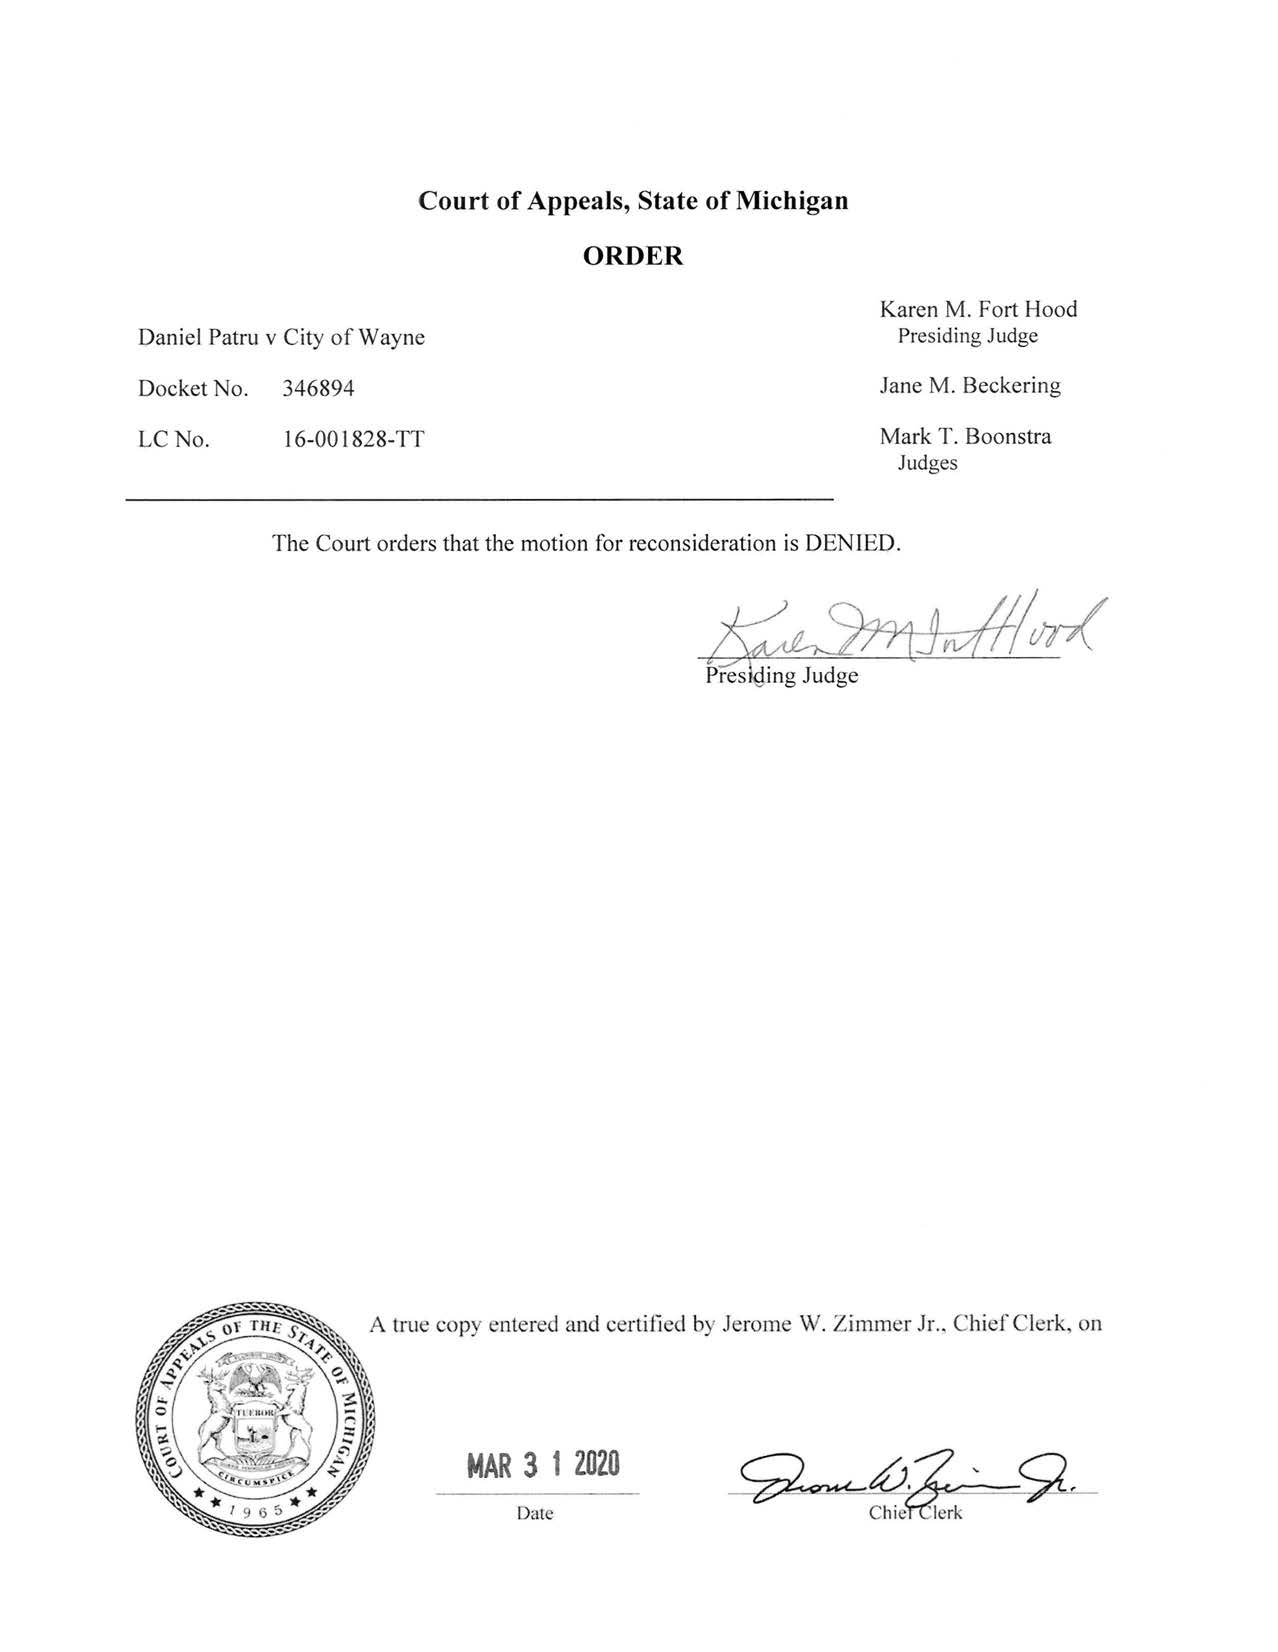
\includepdf[frame,scale=0.7,pagecommand={},pages=-]{appendix/patru2-reconsiderationDenied.pdf}
% \section{Copy of Court of Appeals' 2nd Opinion (2020)}
% 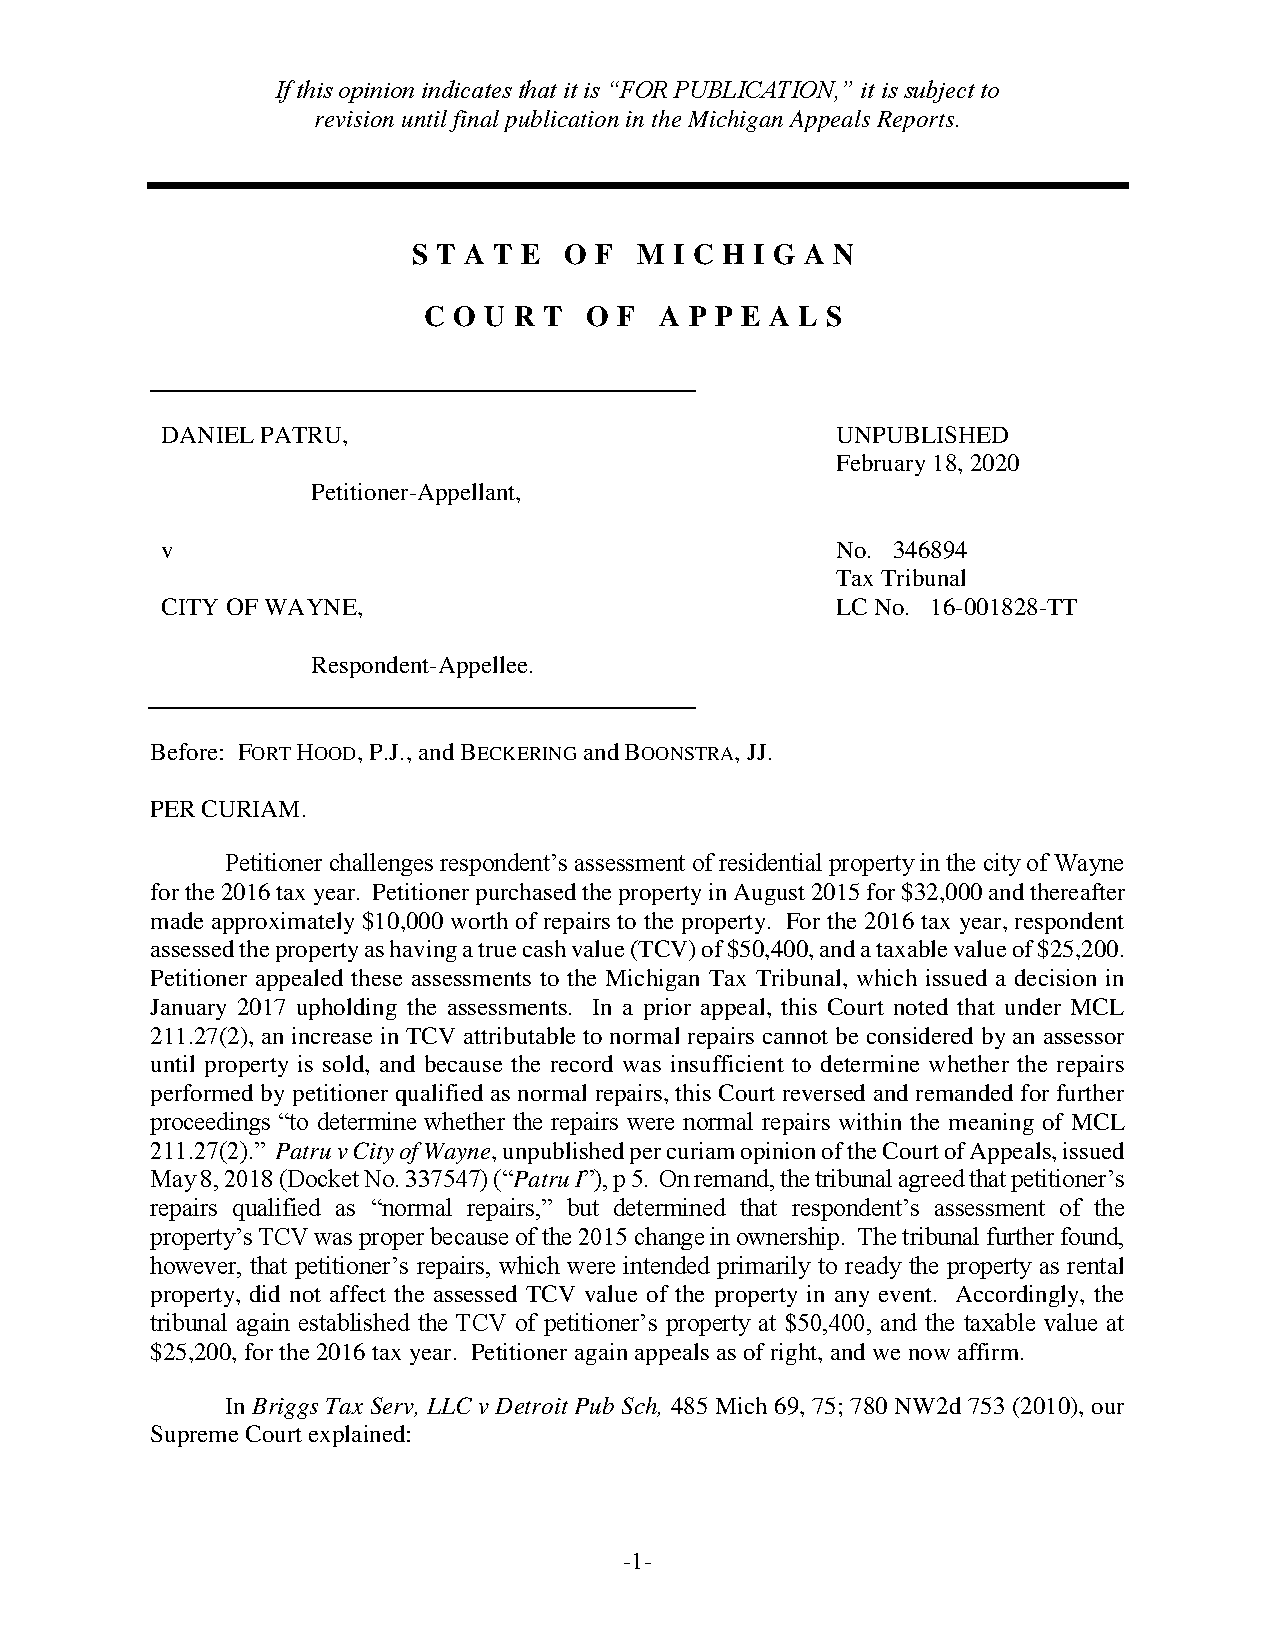
\includepdf[pages=-]{appendix/patru2.pdf}
% \section{Copy of Court of Appeals' 1st Decision (2018)}
% 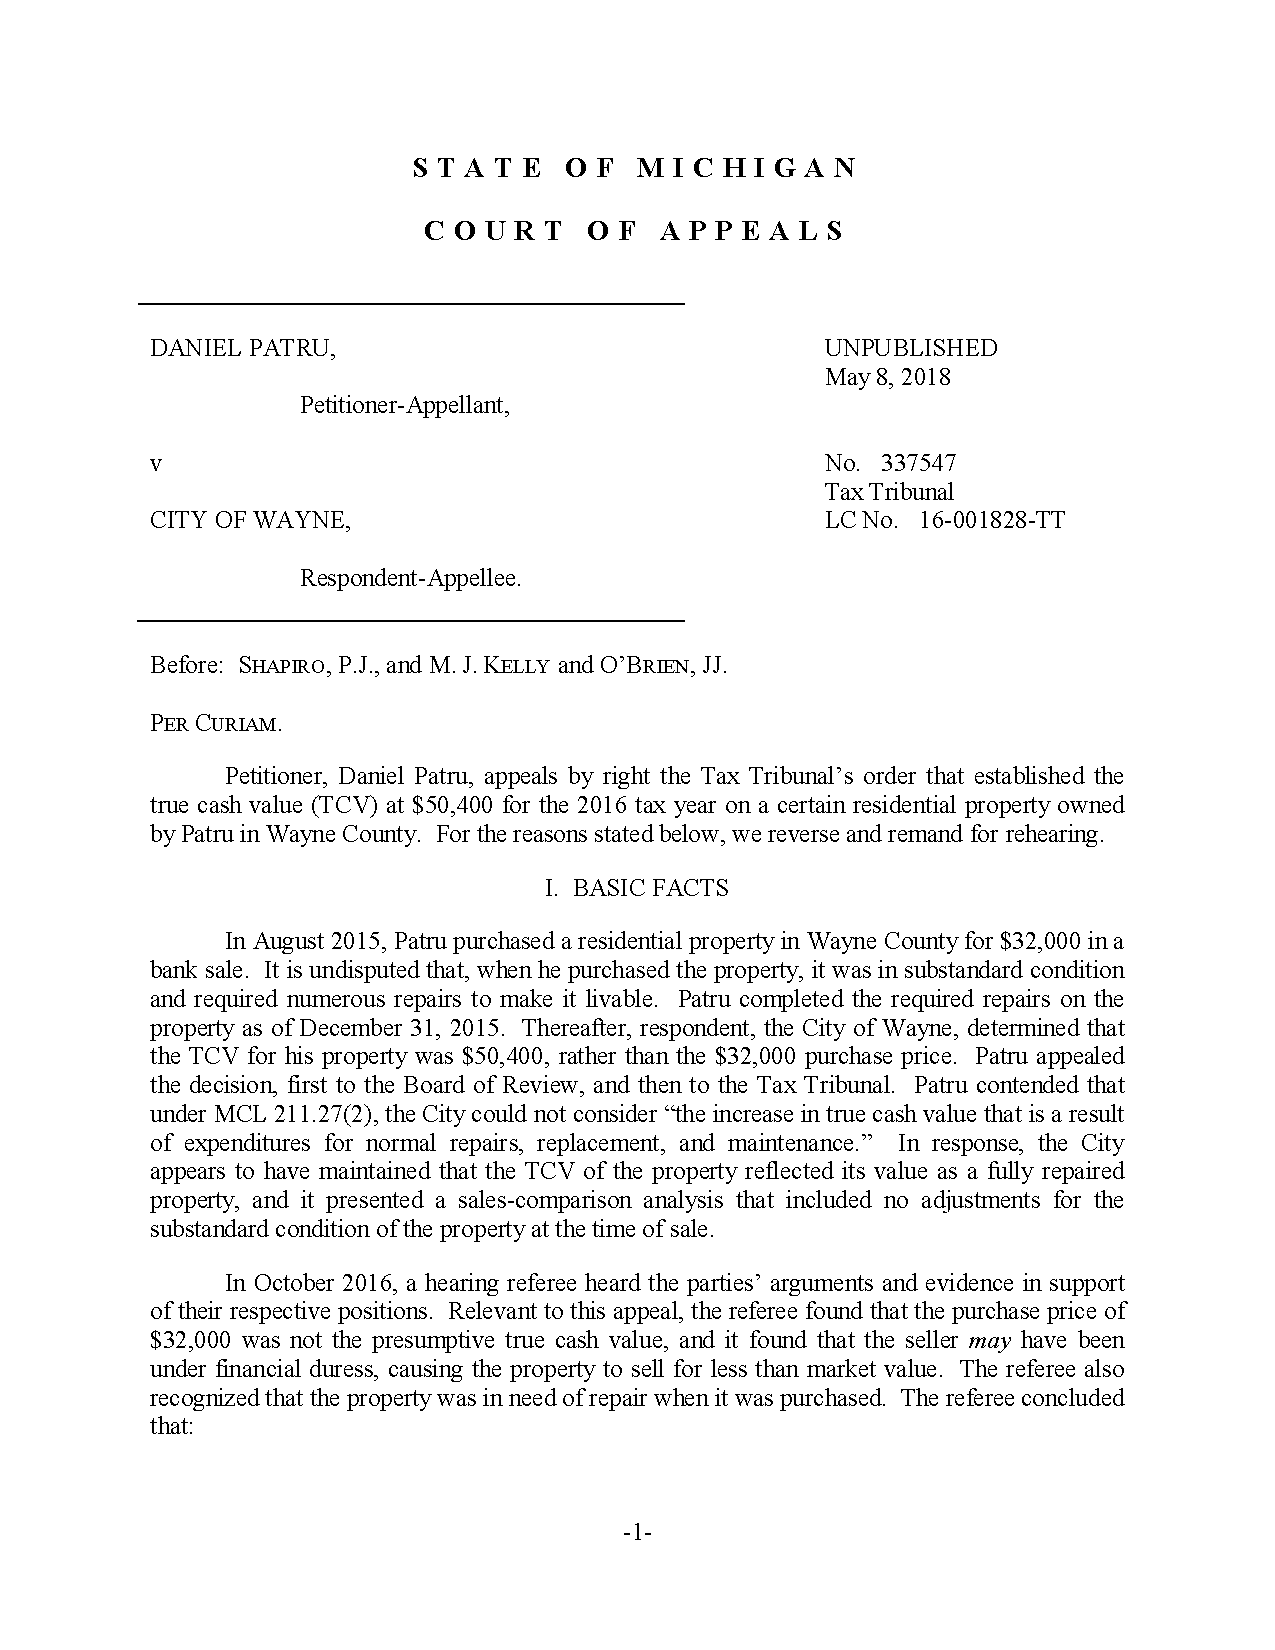
\includepdf[pages=-]{appendix/patru1.pdf}

\end{document}


%%% Local Variables:
%%% mode: latex
%%% TeX-master: t
%%% End:
\end{document}
